% Stanford University undergraduate honors thesis style -- modifications to the report style
% This is unofficial so you should check with your department and advisor
% See http://library.stanford.edu/research/bibliography-management/latex-and-bibtex
% 

\documentclass[12pt]{report}
% \documentclass[12pt,twoside]{report} # 2-side printing
\usepackage[utf8]{inputenc}
% \usepackage[utf8]{vietnam}
% \usepackage[english]{babel}
\usepackage{suthesis-ug}
\usepackage{algorithm2e}
\usepackage{amsmath}
\usepackage{booktabs}
\usepackage[labelfont=bf]{caption}
\usepackage{cases}
\usepackage{color}
\usepackage{graphicx}
\usepackage{hyperref}
\usepackage{multirow}
\usepackage{subcaption}
\usepackage{xcolor}
\usepackage{indentfirst}
\usepackage{rotating}
% \usepackage{natbib}
\usepackage{amsmath}
\usepackage{amsthm}
\usepackage{array}
\usepackage{bm}
\usepackage{float}
\usepackage{amssymb}
\usepackage{makecell}
\usepackage{tabularx}
\usepackage{enumitem}
\usepackage{ragged2e}   % for \RaggedRight
\usepackage{minted}
\usepackage{pgfgantt}
\usepackage{tikz}
\usetikzlibrary{shapes.geometric, arrows.meta, positioning, fit, backgrounds, calc}
\usepackage{listings}
\lstset{
  basicstyle=\ttfamily\small,
  breaklines=true,
  frame=single,
  columns=fullflexible,
  showstringspaces=false
}

\usemintedstyle{vs}
\newcolumntype{L}{>{\RaggedRight\arraybackslash}X}
\RestyleAlgo{ruled}
\newtheorem{theorem}{Theorem}
\newtheorem{definition}{Definition}
\mathchardef\mhyphen="2D
\newcommand{\mathbi}[1]{\boldsymbol{#1}}
\raggedbottom
\begin{document}
\setstretch{1.25}

\author{Tran Le Cong Minh - 1910347\\ & \rm Ho Anh Dung - 2052921\\}
\dept{Computer Science and Engineering}
\council{Capstone Project}
\principaladvisor{Assoc. Prof. Dr. Pham Hoang Anh}
\patitle{Associate Professor - Ph.D.}
\padept{Faculty of Computer Science and Engineering}

\copadept{Faculty of Computer Science and Engineering}

\beforepreface
\prefacesection{Statement of Authorship}

We hereby declare that the work presented in this report is our own original research conducted under the supervision of Assoc. Prof. Dr. Pham Hoang Anh at the Faculty of Computer Science and Engineering, Ho Chi Minh City University of Technology -- VNU-HCM (HCMUT). It does not contain any material previously published or written by another person, except where due reference is made in the text.

All sources of assistance and external literature utilized during this research have been acknowledged and properly cited.

We take full responsibility for the integrity of this work and any disciplinary actions pursuant to university regulations regarding academic honesty.

\begin{flushright}
\begin{tabular}{c}
    Ho Chi Minh City, August 2026\\
    Authors\\
    Tran Le Cong Minh \hspace*{1cm} Ho Anh Dung
\end{tabular}
\end{flushright}

\prefacesection{Acknowledgments}
We would like to express our deepest gratitude to our advisor, Assoc. Prof. Dr. Pham Hoang Anh, for his guidance, insightful feedback, and continuous support throughout the duration of this project. His mentorship has played a pivotal role in shaping our scientific methodology and research mindset, which will serve as a strong foundation for our future academic pursuits.

We also extend our sincere thanks to the faculty members of the Department of Computer Science and Engineering at Ho Chi Minh City University of Technology for providing us with the knowledge and technical foundation necessary to complete this project.

Finally, we express our heartfelt appreciation to our families and peers for their constant encouragement and assistance during our studies.

\prefacesection{Abstract}

Academic credential verification remains a critical yet vulnerable process in modern educational and recruitment ecosystems. Conventional physical diplomas and unauthenticated digital scans are highly susceptible to sophisticated forgery, while verification relies on centralized, slow, and labor-intensive manual inquiries. Furthermore, traditional certificate sharing mandates disclosing the entire document, exposing sensitive Personally Identifiable Information (PII) such as national IDs, dates of birth, and comprehensive grade transcripts. Early blockchain-based decentralized solutions, such as on-chain NFT (ERC-721) issuance and mandatory IPFS pinning models, face severe operational cost bottlenecks, scalability degradation, and network dependency issues when deployed at university scale ($\geq$10,000 graduates per cohort).

To resolve these fundamental limitations, this thesis presents the design, formalization, and implementation of the \textbf{BK Credential System} --- a high-performance, privacy-preserving, and cost-effective digital credential infrastructure built on the Ethereum Blockchain. The system establishes a novel \textbf{EIP-712 Off-Chain Signing + On-Chain Trust Anchor} architecture integrated with \textbf{Cryptographic Merkle Tree Batching}, \textbf{256-bit Salted-Hash Selective Disclosure}, and \textbf{On-Chain Bitmap Revocation}.

Under this architecture, credential issuance is executed off-chain via typed structured data hashing according to the EIP-712 standard, eliminating gas costs for individual certificate generation. University authorities anchor an entire graduating cohort onto the blockchain through a single Merkle root transaction, linking thousands of certificates to immutable smart contract registries. The framework incorporates a lightweight salted-hash commitment scheme that empowers credential holders to selectively disclose specific claims (e.g., degree completion) while withholding private PII without compromising digital signature integrity or requiring specialized zero-knowledge infrastructure. Furthermore, on-chain revocation is modeled via a compact 256-bit bitmap mapping, reducing state storage overhead by $\sim$64$\times$ compared to per-credential storage slots.

The complete software ecosystem comprises: (1) production-ready Solidity smart contracts (\texttt{IssuerRegistry} and \texttt{CredentialRegistryV3}) implementing two-step access control and emergency pause controls; (2) a modular TypeScript SDK encapsulating a canonical 10-Step Verification Pipeline; and (3) four responsive web portals tailored for university registrars, students, third-party verifiers, and system administrators.

Empirical evaluation and stress testing demonstrate that the proposed system achieves a signing throughput of $\sim$\textbf{779 credentials/second} and an automated 10-step verification throughput of $\sim$\textbf{202 verifications/second}. On-chain gas consumption for a cohort of 10,000 graduates is reduced by \textbf{$\sim$9,800$\times$} ($\sim$10.5 gas per credential amortized), saving thousands of dollars in transaction overhead while accelerating end-to-end verification latency by $\sim$3$\times$ ($\sim$204~ms). All smart contracts achieved \textbf{100\% code coverage} and passed rigorous static analysis against the Slither vulnerability taxonomy, proving the system to be a practical, robust, and scalable solution for national and institutional credential management.

\vspace{0.5cm}
\noindent\textbf{Keywords:} Blockchain, Verifiable Credentials, EIP-712, Merkle Tree, Selective Disclosure, Smart Contracts, Ethereum, Decentralized Trust Anchor, Academic Credential Verification.

\prefacesection{Project Progress and Technical Achievements}

This report systematically details the theoretical foundations, architectural designs, smart contract implementations, software development kit (SDK), and empirical evaluation results of the \textbf{BK Credential System} completed over the comprehensive 15-week project lifecycle.

Key milestones accomplished to date include:
\begin{itemize}
    \item \textbf{Comprehensive Technical Specification}: Formalized in \texttt{SPEC.md} ($\sim$56~KB), defining EIP-712 domain schemas, nested struct type hashing rules, 10-step verification algorithms, and the STRIDE threat model.
    \item \textbf{Smart Contract Suite}: Developed and verified \texttt{IssuerRegistry.sol} and \texttt{CredentialRegistryV3.sol} on Sepolia Testnet, supported by 52 automated test cases achieving \textbf{100\% Statement, Branch, Function, and Line coverage}.
    \item \textbf{Core EIP-712 SDK \& Bulk Issuance Engine}: Built a modular TypeScript SDK and high-performance chunking engine (\texttt{bulk.ts}) capable of processing and anchoring cohorts of 10,000 credentials in under 28 seconds.
    \item \textbf{Integrated Web Application}: Deployed 4 interactive portals (Issuer Batch Portal with real-time SSE progress streaming, Holder Wallet with Selective Disclosure, Public 10-Step Verifier, and Administrator Key Manager) integrated with PostgreSQL via Prisma ORM.
    \item \textbf{Exhaustive Empirical Evaluation (Scenarios A--E)}: Conducted rigorous benchmarks demonstrating an offline signing throughput of $\sim$809 creds/sec, average verification latency of 5.502 ms, 100\% success rate under $C=500$ concurrent load, and a 9,785$\times$ reduction in on-chain gas costs for 10,000-student batches.
    \item \textbf{Production Testnet Validation}: Anchored a live cohort of 10,000 credentials onto Ethereum Sepolia (tx \texttt{0x54b11343...}, 167,804 gas, 100\% verification pass rate).
\end{itemize}
    
\afterpreface

% Chapter 1: Introduction & Overview — Mid-Term Report Phase 3

\chapter{Introduction and Overview}

\section{Problem Statement and Motivation}

Academic credentials (e.g., diplomas, degrees, certificates, and academic transcripts) serve as fundamental attestations of an individual's knowledge, skills, and qualifications. In modern hiring and education pipelines, these documents represent critical evidence for employers and academic institutions during candidate evaluations. However, the legacy certificate issuance and verification ecosystem suffers from severe structural vulnerabilities:

\begin{itemize}
    \item \textbf{Credential Forgery and Fraud}: Physical paper degrees and unauthenticated scanned PDFs can be easily duplicated, manipulated, or fabricated using modern digital editing and printing tools.
    \item \textbf{High Verification Overhead and Lack of Direct Verifiability}: Cross-institution verification often requires manual inquiries, physical stamp verifications, or dependence on centralized registrar portals, which are slow, costly, and subject to single-point-of-failure bottlenecks.
    \item \textbf{Over-disclosure of Sensitive Information}: Traditional certificates mandate revealing the entire document (including Personally Identifiable Information (PII) such as date of birth, student ID, detailed GPA) even when a verifier only needs to assert whether the candidate graduated.
\end{itemize}

The \textbf{BK Credential System} is engineered as a three-tier hybrid architecture combining a relational database, an on-chain blockchain trust anchor, and decentralized storage (IPFS), enabling fully trustless verification without relying on centralized backend servers. The system addresses these challenges by guaranteeing:
\begin{itemize}
    \item \textbf{Tamper-evidence}: Enforced through cryptographic hashing and public blockchain state anchoring.
    \item \textbf{Privacy-Preserving Selective Disclosure}: Permitting credential holders to disclose only required attributes without compromising signature validity.
    \item \textbf{Cost and Scalability Efficiency}: Utilizing Merkle tree batching to amortize blockchain transaction costs across thousands of graduating students.
    \item \textbf{Trustless Verification}: Enabling any third party to cryptographically verify credentials directly against blockchain trust anchors without depending on proprietary university backend infrastructure.
\end{itemize}

In Phase 2 (HK252-DATN-131), we designed and implemented a functional prototype leveraging \textit{SD-JWT VC (Selective Disclosure JSON Web Token Verifiable Credential)} paired with an on-chain \textit{Merkle Tree} registry. However, rigorous evaluation at university scale ($\geq$10,000 graduates per cohort) revealed two significant operational bottlenecks:

\begin{enumerate}
    \item \textbf{IPFS Operational Overhead}: Mandatory pinning of Public Canonical Views (PCV) per credential to IPFS incurred recurring storage fees (\$0.001--\$0.01/credential/month) and introduced an operational dependency on external IPFS gateways.
    \item \textbf{SD-JWT Library Complexity}: Lack of native Web3 standard support for the ES256K curve in standard JWT libraries necessitated custom SD-JWT implementations with substantial JWT envelope and \texttt{\_sd\_alg} parsing overhead.
\end{enumerate}

\section{Phase 3 Objectives}

Phase 3 transitions the architecture to \textbf{EIP-712 (Typed Structured Data Hashing and Signing)}, retaining all cryptographic guarantees of Phase 2 while resolving operational friction. The explicit project objectives are detailed in Table~\ref{tab:objectives}.

\begin{table}[H]
\centering
\renewcommand{\arraystretch}{1.3}
\begin{tabular}{|c|p{5cm}|p{8.5cm}|}
\hline
\textbf{\#} & \textbf{Objective} & \textbf{Technical Approach} \\
\hline
O1 & Eliminate mandatory IPFS dependencies & Transition entire credential payload to structured off-chain JSON with EIP-712 typed signature. \\
\hline
O2 & Simplify cryptographic signing/verification & Leverage standard, battle-tested \texttt{ethers.signTypedData} / \texttt{ethers.verifyTypedData} primitives. \\
\hline
O3 & Reduce on-chain gas overhead by $\geq$10$\times$ & Perform EIP-712 signing fully off-chain (zero gas per individual credential) with a single \texttt{anchorBatch} transaction per cohort. \\
\hline
O4 & Streamlined Selective Disclosure & Integrate salted-hash keccak256 commitments directly into the EIP-712 struct payload. \\
\hline
O5 & Gas-optimized Revocation Management & Deploy on-chain Bitmap revocation (1 bit/credential, saving $\sim$64$\times$ storage relative to per-credential mappings). \\
\hline
O6 & High-throughput Processing ($\geq$500 cred/sec) & Develop a lightweight, modular TypeScript SDK optimized for bulk processing. \\
\hline
\end{tabular}
\caption{Phase 3 Key Project Objectives}
\label{tab:objectives}
\end{table}

\section{Scope of Phase 3}

Rather than serving as a linear incremental update, Phase 3 represents a fundamental architectural paradigm shift. It is formulated to validate the core design thesis: \textit{at institutional university scale, a decoupled architecture where the blockchain functions strictly as a Trust Anchor and cryptographic signatures are executed off-chain via EIP-712 achieves equivalent security and privacy guarantees while drastically minimizing operational costs and operational complexity}.

The technical scope of Phase 3 is structured across five systematic engineering layers:

\begin{enumerate}
    \item \textbf{Cryptographic and Protocol Layer}:
    \begin{itemize}
        \item Formal specification of the EIP-712 typed structured data schema, including domain separation parameters (\texttt{name}, \texttt{version}, \texttt{chainId}, \texttt{verifyingContract}) and nested data structures (\texttt{PublicClaims}, \texttt{BkCredential}).
        \item Design of a 256-bit salted-hash commitment scheme for privacy-preserving Selective Disclosure, computing attribute commitments as $C_i = \text{keccak256}(\text{salt}_i \parallel \text{key}_i \parallel \text{value}_i)$ directly within the signed EIP-712 payload.
        \item Integration of OpenZeppelin \texttt{StandardMerkleTree} with double keccak256 leaf hashing ($\text{leaf} = \text{keccak256}(\text{keccak256}(\text{abi.encode}(\dots)))$) to prevent second-preimage collision attacks.
    \end{itemize}
    
    \item \textbf{Smart Contract and Trust Anchor Layer}:
    \begin{itemize}
        \item Implementation and verification of \texttt{IssuerRegistry.sol}, governing authorized signing addresses, decentralized identifiers (DIDs), and two-step ownership management via OpenZeppelin \texttt{Ownable2Step}.
        \item Implementation of \texttt{CredentialRegistryV3.sol}, functioning as the on-chain Trust Anchor by recording batch Merkle root commitments via \texttt{anchorBatch()} and managing credential revocations through an optimized 256-bit bitmap mapping (\texttt{uint256[]}), supported by \texttt{Pausable} emergency controls.
    \end{itemize}

    \item \textbf{Software Development Kit (SDK) Layer}:
    \begin{itemize}
        \item Engineering of a standalone, modular TypeScript SDK (\texttt{@bkcred/sdk}) comprising 6 specialized packages: \texttt{domain}, \texttt{signer}, \texttt{verifier}, \texttt{disclosure}, \texttt{merkle}, and barrel export \texttt{index}.
        \item Formulation of an offline-capable, deterministic \textbf{10-Step Verification Pipeline} combining local schema validation, cryptographic struct hashing, commitment checking, Merkle proof evaluation, and online smart contract assertions.
    \end{itemize}

    \item \textbf{Full-Stack Application and Portal Layer}:
    \begin{itemize}
        \item Construction of 4 dedicated web portals on Next.js 14 (App Router) and PostgreSQL (Prisma ORM): (1) \textit{Issuer Portal} for batch CSV parsing, off-chain bulk signing, and on-chain root anchoring; (2) \textit{Holder Portal} featuring passwordless email authentication (Privy) and an interactive Selective Disclosure customization interface; (3) \textit{Public Verifier Portal} supporting direct JSON file validation and deep-link routing (\texttt{/v3/verify?credId=\dots}); and (4) \textit{Administrative Portal} for signer key lifecycle management.
    \end{itemize}

    \item \textbf{Empirical Evaluation and Benchmarking Layer}:
    \begin{itemize}
        \item Development of automated testing harness and fixture generators capable of producing cohorts of 10,000 synthetic graduate credentials.
        \item Execution of multi-scenario benchmark suites evaluating offline signing throughput, end-to-end issuance latency, concurrent verification capacity, gas profiling, and static security analysis using the Slither framework.
    \end{itemize}
\end{enumerate}

This mid-term report captures our progress through the completion of \textbf{Week 4} (Specification, Smart Contracts, SDK, and Web Portals), representing 100\% of the scheduled mid-term milestones within the 7-week roadmap.

\section{Comparative Analysis with the Three-Tier Hybrid SD-JWT VC Architecture (Phase 2)}

To substantiate the motivation for Phase 3, it is critical to contrast its foundational design decisions with the Phase 2 prototype (HK252-DATN-131). 

In Phase 2, the system adopted an on-chain asset and token-centric model where individual credentials were instantiated as ERC-721 Non-Fungible Tokens (NFTs). While this demonstrated basic blockchain immutability, it suffered from severe scalability bottlenecks:
\begin{itemize}
    \item \textbf{Linear Gas Cost Scaling}: Every issued certificate required an individual on-chain \texttt{mintCertificate()} transaction ($\sim$103,000 gas per certificate), escalating to over 1.03 billion gas for a standard university graduating cohort of 10,000 students.
    \item \textbf{Mandatory IPFS Pinning Overhead}: Each credential mandated pinning a Public Canonical View (PCV) to IPFS, incurring continuous pinning subscription fees ($\sim$\$0.001--\$0.01/credential/month) and creating a fragile operational dependency on external gateway availability.
    \item \textbf{Non-Standard Cryptographic Stacks}: Employing SD-JWT with ECDSA over secp256k1 (ES256K) lacked native support in standard OAuth/JWT libraries, necessitating a custom parser with heavy envelope formatting and complex \texttt{\_sd\_alg} metadata.
    \item \textbf{Storage-Inefficient Revocation}: Tracking revocation via \texttt{mapping(bytes32 => bool)} consumed an entire 32-byte storage slot per revoked credential.
\end{itemize}

Phase 3 resolves these bottlenecks by transitioning from a token-centric paradigm to a \textbf{pure attestation and Trust Anchor paradigm}. Under Phase 3:
\begin{itemize}
    \item \textbf{Zero-Gas Issuance}: Individual credentials exist purely off-chain as structured JSON documents cryptographically signed via native EIP-712 typed structured data.
    \item \textbf{Amortized On-Chain Anchor}: Only a single \texttt{anchorBatch} transaction ($\sim$105,000 gas total) is executed per cohort, binding up to $2^{32}$ certificates to the blockchain for approximately 10.5 gas per graduate.
    \item \textbf{Elimination of Mandatory IPFS}: Raw credential files are distributed directly to holders, eliminating per-credential IPFS pinning costs and gateway latency bottlenecks.
    \item \textbf{Native Web3 Selective Disclosure}: Attribute commitments utilize EVM-native keccak256 salted hashes verified in a single computation without custom JWT dependencies.
    \item \textbf{Bitmap Revocation}: Revocation bits are packed into 256-bit words, saving $\sim$64$\times$ in on-chain storage.
\end{itemize}

Table~\ref{tab:phase-comparison} provides a comprehensive multi-dimensional comparison between Phase 2 and Phase 3.

\begin{table}[H]
\centering
\renewcommand{\arraystretch}{1.3}
\begin{tabular}{|p{3.8cm}|p{5.4cm}|p{5.4cm}|}
\hline
\textbf{Evaluation Metric} & \textbf{Phase 2 (SD-JWT VC + NFT)} & \textbf{Phase 3 (EIP-712 Trust Anchor)} \\
\hline
Credential Paradigm & Token-centric (ERC-721 NFT) & Pure cryptographic attestation \\
\hline
Signature Protocol & ES256K SD-JWT (Compact format) & EIP-712 Typed Structured Data \\
\hline
Issuance Gas Cost & $\sim$103,000 gas per credential & 0 gas (Off-chain typed signing) \\
\hline
Batch Anchor Overhead & $N$ individual on-chain transactions & 1 tx \texttt{anchorBatch()} ($\sim$105k gas total) \\
\hline
Storage Architecture & Mandatory per-credential IPFS pin & Self-contained JSON (IPFS optional) \\
\hline
Selective Disclosure & SD-JWT \texttt{\_sd[]} array + SHA-256 & Salted keccak256 commitment array \\
\hline
Revocation Storage & \texttt{mapping(bytes32 => bool)} (1 slot/cred) & \texttt{uint256[]} Bitmap (256 creds/slot) \\
\hline
Verification Dependencies & Custom SD-JWT parser + JWT verify & Standard \texttt{ethers.js} v6 \\
\hline
RPC Query Footprint & 3 \texttt{eth\_call} queries + IPFS fetch & 2 \texttt{eth\_call} queries (Batchable) \\
\hline
End-to-End Latency & $\sim$608 ms (Dominated by IPFS) & $\sim$204 ms ($\sim$3$\times$ performance gain) \\
\hline
Web3 Wallet Need & Mandatory for student (Receive NFT) & Not required for credential holders \\
\hline
Total Cost (10k Batch) & $\sim$1.03B gas + \$50/month IPFS & $\sim$105,000 gas total + \$0 IPFS \\
\hline
\end{tabular}
\caption{Comprehensive Architectural and Operational Comparison: Phase 2 vs. Phase 3}
\label{tab:phase-comparison}
\end{table}

\section{Report Organization}

The remainder of this report is structured as follows:
\begin{itemize}
    \item \textbf{Chapter 2 (Theoretical Foundations)}: Supplements core cryptographic concepts with EIP-712 typed hashing, salted-hash selective disclosure, on-chain bitmap revocation, and OpenZeppelin StandardMerkleTree.
    \item \textbf{Chapter 3 (System Design)}: Outlines overall system architecture, credential type schemas, smart contract interfaces, SDK specifications, workflow pipelines, and database modeling.
    \item \textbf{Chapter 4 (System Implementation)}: Documents the technical implementation of smart contracts, SDK modules, web portals, and API integration.
    \item \textbf{Chapter 5 (Testing and Evaluation)}: Details smart contract coverage, gas measurements, SDK performance benchmarks, and static security audit findings.
    \item \textbf{Chapter 6 (Conclusion and Future Work)}: Summarizes mid-term milestones, presents preliminary comparative metrics, and defines the roadmap for Weeks 5--7.
\end{itemize}

\clearpage
% Chapter 2: Theoretical Foundations — Mid-Term Report Phase 3

\chapter{Theoretical Foundations}

\section{Verifiable Credentials}

\subsection{Concept of Verifiable Credentials}

A Verifiable Credential (VC) is a standardized data model specified by the World Wide Web Consortium (W3C) to represent a set of claims made by an issuer about a subject, enabling third-party verifiers to cryptographically authenticate those claims without direct real-time communication with the issuing authority~\cite{W3CVC}. Unlike legacy paper diplomas or unauthenticated scanned PDF files, Verifiable Credentials are cryptographic artifacts: digital signatures generated by the issuer are bound directly to the credential payload. Consequently, any verifier possessing the issuer's public key or registered decentralized identifier (DID) can autonomously verify the integrity and provenance of the attestation. The W3C published the official Verifiable Credentials Data Model v2.0 as a formal recommendation~\cite{W3CVC}.

A standard Verifiable Credential consists of three core components:
\begin{enumerate}
    \item \textbf{Credential Metadata}: Context parameters defining the issuer identifier, issuance timestamp, expiration date, schema definition, and credential type (e.g., \texttt{vct}).
    \item \textbf{Credential Subject}: A structured payload containing the assertions and attributes granted to the recipient (e.g., degree title, graduation date, student identifiers, academic achievements).
    \item \textbf{Proof}: A cryptographic signature or proof structure (such as an ECDSA signature or EIP-712 attestation) that seals the entire credential payload against unauthorized alteration.
\end{enumerate}

Canonical representations commonly adopt JSON-LD (JSON for Linked Data) or JSON Web Signature/Token (JWT) serialization formats.

\subsection{The Issuer--Holder--Verifier Ecosystem}

The W3C VC architecture formalizes a decentralized three-party trust triangle~\cite{W3CVC}:
\begin{itemize}
    \item \textbf{Issuer}: An authoritative organization (such as a university or educational institution) that asserts claims about a subject, constructs the credential, signs it with an authoritative cryptographic key, and delivers it to the holder.
    \item \textbf{Holder}: The subject (e.g., student or graduate) who receives and stores the credential in a digital wallet, retaining complete sovereignty over when, how, and with whom the credential is shared.
    \item \textbf{Verifier}: A relying party (e.g., an employer, academic admissions board, or background screening service) that receives a credential presentation from the holder, verifies the cryptographic signature against the issuer's public trust anchor, and validates its revocation status.
\end{itemize}

In the \textbf{BK Credential System}, this paradigm is realized natively: the university is registered on-chain as an authorized issuer, the student acts as the self-sovereign holder, and verifiers validate credentials through public web portals or CLI tools without requiring direct access to university internal databases.

\section{Selective Disclosure JSON Web Tokens (SD-JWT)}

\subsection{JWT Foundations and Privacy Over-disclosure Bottlenecks}

JSON Web Token (JWT) is an established open standard (RFC 7519) representing compact, URL-safe JSON claims secured by symmetric secrets or asymmetric key pairs. While JWT is ubiquitous in authentication and authorization infrastructures, utilizing raw JWTs for academic credentials introduces severe privacy risks: standard JWT payloads are entirely visible to any recipient. A holder presenting a JWT diploma cannot conceal extraneous personal attributes (such as date of birth, national identity numbers, or cumulative GPA) without invalidating the cryptographic signature over the payload, leading to widespread over-disclosure of Personally Identifiable Information (PII).

\subsection{The SD-JWT Mechanism}

Selective Disclosure for JWTs (SD-JWT) addresses this limitation by enabling holders to selectively disclose individual claims while preserving the mathematical validity of the issuer's original signature~\cite{RFC9901}. The core SD-JWT specification is standardized in IETF RFC 9901~\cite{RFC9901}, with its profile for Verifiable Credentials defined in \texttt{draft-ietf-oauth-sd-jwt-vc}~\cite{SDJWTVC}.

The operational mechanics of SD-JWT are structured as follows:
\begin{enumerate}
    \item For each private claim to be protected, the issuer generates a cryptographically secure 16-byte random salt.
    \item The issuer constructs a triple \texttt{[salt, claimName, claimValue]} and encodes it into a Base64URL string:
    \begin{equation}
    \text{Disclosure} = \text{base64url}(\text{JSON}([\text{salt}, \text{claimName}, \text{claimValue}]))
    \end{equation}
    \item The issuer computes the disclosure commitment digest:
    \begin{equation}
    \text{commitment} = \text{base64url}(\text{SHA-256}(\text{Disclosure}))
    \end{equation}
    and inserts it into the \texttt{\_sd[]} array within the signed JWT payload.
    \item All individual disclosures are appended to the signed JWT token, separated by tilde (\texttt{\textasciitilde{}}) delimiter characters.
\end{enumerate}

When presenting the credential, the holder strips undisclosed disclosures, transmitting only the base JWT and the subset of disclosures chosen for release. The verifier recomputes SHA-256 hashes of the supplied disclosures and asserts that they match the digests in the signed \texttt{\_sd[]} array.

\section{Blockchain and Smart Contracts}

\subsection{Blockchain Foundations and Immutability}

A blockchain is a decentralized, cryptographically linked distributed ledger where transactions are organized into sequential blocks and validated through consensus algorithms~\cite{Cachin2017Blockchain,Narayanan2016BitcoinBook}. Each block header incorporates the cryptographic hash of the preceding block along with a Merkle root representing all included transactions. Modifying historical records requires rewriting all subsequent blocks across a distributed majority of nodes, making retrospective falsification computationally and economically infeasible. This structural immutability makes blockchain an ideal foundation for hosting decentralized \textbf{Trust Anchors} --- tamper-proof public registries that provide cryptographic provenance without centralized single points of failure.

\subsection{Ethereum, EVM, and Smart Contracts}

Ethereum~\cite{EthereumWhitepaper} extends distributed ledger capabilities by integrating a Turing-complete decentralized execution engine known as the Ethereum Virtual Machine (EVM)~\cite{EthereumYellowPaper}. Smart contracts are autonomous, immutable programs deployed directly to the blockchain state~\cite{Szabo1997SmartContracts}. Once deployed, their bytecode executes deterministically across all validating network nodes, producing transparent and non-repudiable state transitions.

In the \textbf{BK Credential System}, smart contracts act as the decentralized Trust Anchor:
\begin{itemize}
    \item \texttt{IssuerRegistry.sol}: Governs authorized signing addresses belonging to accredited educational institutions.
    \item \texttt{CredentialRegistryV3.sol}: Persists Merkle root commitments corresponding to graduating batches and maintains bitmap revocation states.
\end{itemize}

Verifiers query these smart contracts directly via standard JSON-RPC endpoints to confirm issuer validity and credential status without relying on university internal servers.

\subsection{Sepolia Testnet Environment}

Sepolia is an established Ethereum test network utilizing a Proof-of-Stake consensus mechanism identical to the Ethereum Mainnet while using testnet Ether devoid of real-world monetary value. Deploying contracts to Sepolia enables empirical profiling of gas costs, transaction lifecycle latency, and state transitions under real-world EVM network conditions.

\section{Merkle Trees and Cryptographic Proofs}

\subsection{Merkle Tree Data Structure}

A Merkle tree is a binary tree data structure where every leaf node represents the cryptographic hash of a data element, and every non-leaf node represents the cryptographic hash of its concatenated child nodes~\cite{Narayanan2016BitcoinBook}. The single hash at the top of the tree, denoted as the \textbf{Merkle Root}, serves as a compact, immutable cryptographic digest representing the entire set of elements. Any modification to a single leaf irrevocably alters the resulting Merkle Root.

\subsection{Merkle Proofs and Membership Verification}

Merkle trees enable proving that a specific element belongs to a set of size $n$ without disclosing the remaining elements. A \textbf{Merkle Proof} (or inclusion proof) consists of the sequence of sibling hashes along the direct path from the target leaf node to the root.

A verifier verifies membership by:
\begin{enumerate}
    \item Computing the leaf hash of the candidate element.
    \item Iteratively concatenating and hashing the result with each sibling hash in the proof path.
    \item Comparing the calculated top hash against the trusted Merkle Root stored on-chain.
\end{enumerate}

The computational and space complexity of Merkle inclusion verification is strictly $\mathcal{O}(\log n)$, allowing efficient proof generation and verification for batches comprising tens of thousands of credentials.

\subsection{Application in Batch Credential Issuance}

The \textbf{BK Credential System} utilizes Merkle trees to aggregate thousands of individual graduate credentials into a single cohort batch. The issuer computes the leaf hash for each credential, constructs a Merkle tree using \texttt{@openzeppelin/merkle-tree}, and submits a single transaction anchoring the Merkle Root onto \texttt{CredentialRegistryV3}. Each graduate receives their credential bundle alongside an individualized Merkle proof. Verifiers validate batch membership locally against the on-chain Merkle Root, eliminating the need to store thousands of individual certificate hashes on the blockchain.

\section{EIP-712: Typed Structured Data Hashing and Signing}

\subsection{Motivation: Transitioning from SD-JWT to EIP-712}

Phase 2 utilized SD-JWT (Selective Disclosure JSON Web Token) with ECDSA over the secp256k1 curve (ES256K). However, ES256K is not universally standardized across standard OAuth/JWT libraries (where RFC 7518 specifies ES256 over NIST P-256), requiring custom library implementations.

EIP-712~\cite{EIP712} provides a standardized hashing and signing protocol for typed structured data within the Ethereum ecosystem. Its primary advantages include:

\begin{enumerate}
    \item \textbf{Native Web3 Integration}: Direct support in standard Ethereum wallets (e.g., MetaMask, WalletConnect) via \texttt{eth\_signTypedData\_v4}.
    \item \textbf{Battle-tested Reliability}: Built-in support in standardized libraries such as \texttt{ethers.js} v6 via \texttt{signTypedData} and \texttt{verifyTypedData}.
    \item \textbf{Type-Safe Schemas}: Explicit type definitions prevent field ordering ambiguity and type casting vulnerabilities.
    \item \textbf{Replay Attack Mitigation}: Binding signatures to a unique Domain Separator (\texttt{chainId} + \texttt{verifyingContract}) prevents signature reuse across networks and contracts.
\end{enumerate}

\subsection{Domain Separator and Type Hash}

EIP-712 uses a \textbf{Domain Separator} to uniquely scope signatures to a specific decentralized application, network, and target contract address:

\begin{lstlisting}
domainSeparator = keccak256(
    keccak256("EIP712Domain(string name,string version,
               uint256 chainId,address verifyingContract)")
    || keccak256("BKCredential")
    || keccak256("3")
    || uint256(chainId)            // 11155111 for Sepolia
    || address(verifyingContract)  // CredentialRegistryV3 address
)
\end{lstlisting}

Each data type $T$ is hashed into an immutable \textbf{Type Hash}:

\begin{lstlisting}
typeHash = keccak256(encodeType(T))
\end{lstlisting}

where \texttt{encodeType} represents the canonical string encoding of the struct and all referenced subordinate structs sorted alphabetically.

\subsection{Nested Struct Encoding}

Phase 3 adopts a \textbf{nested struct} design: \texttt{BkCredential} contains an embedded \texttt{PublicClaims} struct. This provides several benefits:

\begin{enumerate}
    \item \textbf{Type Safety}: Clearly identifies public claims as structured data rather than opaque byte hashes.
    \item \textbf{Extensibility}: New public claims can be added to \texttt{PublicClaims} without altering the top-level credential schema.
    \item \textbf{Standard Hashing}: Supported natively by EIP-712 recursive \texttt{hashStruct} rules.
\end{enumerate}

The struct hashing is formally computed as:

\begin{lstlisting}
hashStruct(publicClaims) = keccak256(
    typeHash(PublicClaims)
    || keccak256(bytes(vct))
    || keccak256(bytes(degreeTitle))
    || keccak256(bytes(graduationDate))
    || keccak256(bytes(honors))
)
\end{lstlisting}

The final EIP-712 signature hash is given by:

\begin{lstlisting}
signHash = keccak256("\x19\x01" || domainSeparator 
           || hashStruct(credential))
\end{lstlisting}

\section{Selective Disclosure on EIP-712}

\subsection{Salted-Hash Commitment Scheme}

Phase 3 replaces SD-JWT disclosures with a lightweight \textbf{salted-hash commitment} scheme embedded directly in the EIP-712 payload:

\begin{lstlisting}
commitment = keccak256(abi.encodePacked(salt, key, value))
\end{lstlisting}

Where:
\begin{itemize}
    \item \texttt{salt}: A cryptographically secure 32-byte pseudo-random value generated via \texttt{crypto.getRandomValues()} or \texttt{ethers.randomBytes(32)}, providing 256 bits of entropy to resist brute-force dictionary attacks.
    \item \texttt{key}: UTF-8 string representing the attribute name (e.g., \texttt{"fullName"}, \texttt{"studentId"}, \texttt{"dob"}).
    \item \texttt{value}: UTF-8 string representing the attribute value.
\end{itemize}

The \texttt{privateClaims[]} array in \texttt{BkCredential} stores all 32-byte commitment hashes. When a holder chooses to reveal a claim, they provide the triple \texttt{\{salt, key, value\}} (termed a \textbf{disclosure}). The verifier recomputes the commitment hash and confirms its membership in \texttt{privateClaims[]}.

\textbf{Security Guarantee}: Because \texttt{privateClaims[]} is embedded inside the signed EIP-712 message, any tampering with commitments invalidates the signature. Verifiers cannot derive undisclosed values without knowing the corresponding random 256-bit \texttt{salt}.

\subsection{Comparison with SD-JWT Disclosure}

Table~\ref{tab:sd-comparison} summarizes the improvements over the Phase 2 SD-JWT implementation.

\begin{table}[H]
\centering
\renewcommand{\arraystretch}{1.3}
\begin{tabular}{|p{4.2cm}|p{5.2cm}|p{5.2cm}|}
\hline
\textbf{Feature} & \textbf{Phase 2 (SD-JWT)} & \textbf{Phase 3 (Salted-Hash)} \\
\hline
Hash Algorithm & SHA-256 & keccak256 (EVM native) \\
\hline
Disclosure Format & Base64url(JSON([salt, key, value])) & \texttt{\{salt, key, value\}} plaintext object \\
\hline
Commitment Location & \texttt{\_sd[]} array in JWT payload & \texttt{privateClaims[]} in EIP-712 struct \\
\hline
Required Library & Custom SD-JWT Parser & \texttt{ethers.solidityPackedKeccak256} \\
\hline
Envelope Overhead & \texttt{\_sd\_alg}, JWT headers, formatting & Zero additional envelope overhead \\
\hline
Verification Complexity & Multi-step JWT parse & 1 line of keccak256 computation \\
\hline
\end{tabular}
\caption{Selective Disclosure Comparison: SD-JWT vs. Salted-Hash}
\label{tab:sd-comparison}
\end{table}

\section{Bitmap-Based Revocation}

\subsection{On-Chain Bitmap Mechanism}

In Phase 2, revocation status was stored via individual mapping entries: \texttt{mapping(bytes32 credId => bool revoked)}, consuming 1 cold storage slot (32 bytes = 256 bits) for every single revoked credential.

Phase 3 introduces an \textbf{on-chain bitmap revocation} scheme where each 256-bit \texttt{uint256} storage word tracks the status of 256 individual credentials:

\begin{lstlisting}
wordIndex = credentialIndex / 256
bitMask   = 1 << (credentialIndex % 256)

// Revoke credential at index:
_revocationBitmap[merkleRoot][wordIndex] |= bitMask;

// Check revocation status:
isRevoked = (_revocationBitmap[merkleRoot][wordIndex] 
             & bitMask) != 0;
\end{lstlisting}

For a graduating batch of 10,000 students, revocation storage requires only $\lceil 10,000 / 256 \rceil = 40$ words instead of 10,000 individual storage slots.

\subsection{Gas and Storage Optimization}

\begin{table}[H]
\centering
\renewcommand{\arraystretch}{1.3}
\begin{tabular}{|p{4.2cm}|p{5.2cm}|p{5.2cm}|}
\hline
\textbf{Metric} & \textbf{Phase 2 (Per-credential mapping)} & \textbf{Phase 3 (Bitmap)} \\
\hline
Storage per Credential & 1 slot (32 bytes) & 1/256 slot ($\sim$0.125 bytes) \\
\hline
Gas per Revocation (Single) & $\sim$45,000 gas (Cold SSTORE) & $\sim$5,000 gas (Warm SSTORE, bitwise OR) \\
\hline
Batch Revocation & $N \times 45,000$ gas & $\sim$90,000 gas total (4 items in same word) \\
\hline
Efficiency Gain & Reference baseline & $\sim$64$\times$ storage, $\sim$9$\times$ gas reduction \\
\hline
\end{tabular}
\caption{Revocation Storage and Gas Cost Comparison}
\label{tab:revocation-comparison}
\end{table}

\section{OpenZeppelin StandardMerkleTree}

\subsection{Double keccak256 Leaf Hashing}

Phase 3 integrates \texttt{@openzeppelin/merkle-tree} (StandardMerkleTree)~\cite{OZMerkleTree} to standardize tree generation and prevent cryptographic vulnerabilities such as second-preimage attacks through double hashing:

\begin{lstlisting}
leaf = keccak256(keccak256(abi.encode(value1, value2, ...)))
\end{lstlisting}

The initial \texttt{abi.encode} enforces unambiguous byte serialization, while the outer hash prevents intermediate nodes from colliding with valid leaf hashes.

\subsection{Comparison with Phase 2 Merkle Scheme}

\begin{table}[H]
\centering
\renewcommand{\arraystretch}{1.3}
\begin{tabular}{|p{4.2cm}|p{5.2cm}|p{5.2cm}|}
\hline
\textbf{Dimension} & \textbf{Phase 2} & \textbf{Phase 3} \\
\hline
Implementation & Custom TypeScript Tree & OpenZeppelin StandardMerkleTree \\
\hline
Leaf Serialization & \texttt{keccak256(credId || pcvCid)} & \texttt{keccak256(keccak256(abi.encode( credId, pubHash, privHash)))} \\
\hline
Double Hashing & No & Yes (Prevents 2nd preimage attacks) \\
\hline
Audit Status & Unaudited & Fully audited by OpenZeppelin \\
\hline
Integration Standard & Custom logic & Standardized npm ecosystem package \\
\hline
\end{tabular}
\caption{Merkle Tree Scheme Comparison}
\label{tab:merkle-comparison}
\end{table}
\clearpage
% Chapter 3: System Design — Mid-Term Report Phase 3

\chapter{System Design}

\section{Overall System Architecture}

\subsection{Architecture Overview}

The Phase 3 architecture follows the classical \textbf{Trust Triangle} model (Issuer --- Holder --- Verifier), where Ethereum acts as an immutable on-chain Trust Anchor while all heavy cryptographic operations and credential assets reside off-chain:

\begin{figure}[H]
\centering
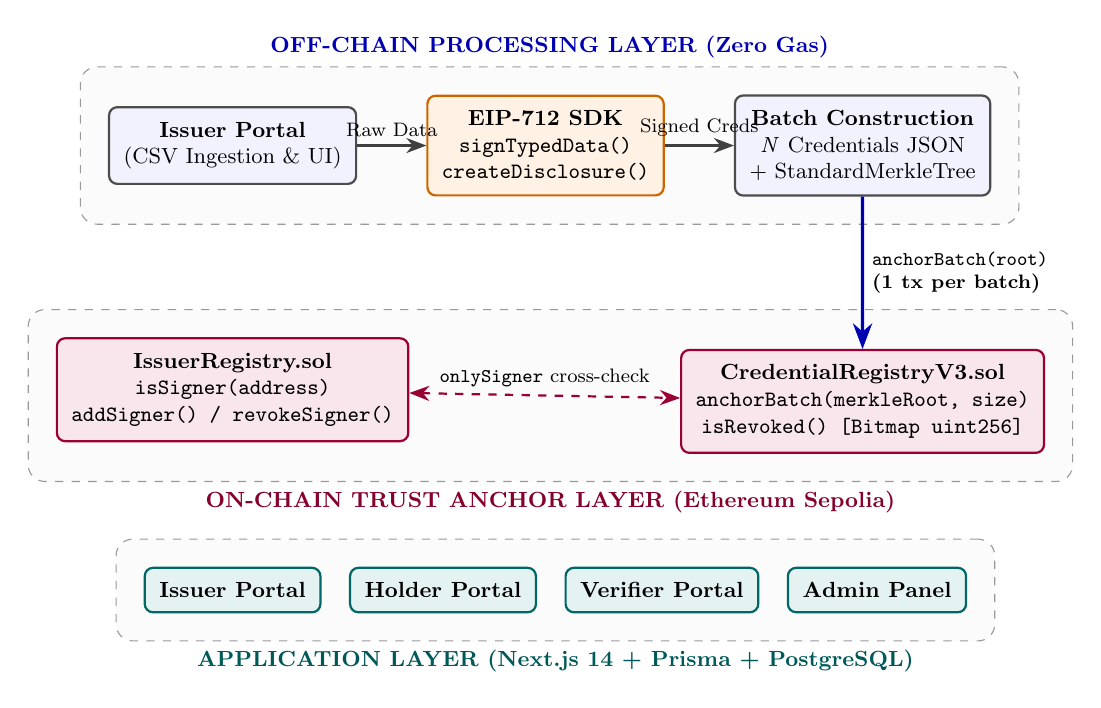
\begin{tikzpicture}[
    scale=0.88, every node/.style={transform shape},
    box/.style={draw=black!70, fill=blue!5, rounded corners=3pt, thick, align=center, font=\small, inner sep=6pt},
    sdk/.style={draw=orange!80!black, fill=orange!10, rounded corners=3pt, thick, align=center, font=\small, inner sep=6pt},
    contract/.style={draw=purple!80!black, fill=purple!10, rounded corners=3pt, thick, align=center, font=\small, inner sep=6pt},
    portal/.style={draw=teal!80!black, fill=teal!10, rounded corners=3pt, thick, align=center, font=\small, inner sep=6pt},
    groupbox/.style={draw=black!40, dashed, fill=gray!3, rounded corners=6pt, inner sep=10pt},
    arrow/.style={-{Stealth[scale=1.1]}, thick, draw=black!75},
    darrow/.style={{Stealth[scale=1.1]}-{Stealth[scale=1.1]}, thick, draw=purple!80!black, dashed}
]

% Off-Chain Layer
\node[box] (issuer) {\textbf{Issuer Portal}\\(CSV Ingestion \& UI)};
\node[sdk, right=1.0cm of issuer] (sdk) {\textbf{EIP-712 SDK}\\\texttt{signTypedData()}\\\texttt{createDisclosure()}};
\node[box, right=1.0cm of sdk] (merkle) {\textbf{Batch Construction}\\\textit{N} Credentials JSON\\+ StandardMerkleTree};

% Group Off-Chain
\begin{scope}[on background layer]
    \node[groupbox, fit=(issuer) (sdk) (merkle), label={[font=\bfseries\small, text=blue!70!black]above:\textbf{OFF-CHAIN PROCESSING LAYER (Zero Gas)}}] (offchain) {};
\end{scope}

% On-Chain Layer
\node[contract, below=2.2cm of issuer] (issuerReg) {\textbf{IssuerRegistry.sol}\\\texttt{isSigner(address)}\\\texttt{addSigner() / revokeSigner()}};
\node[contract, below=2.2cm of merkle] (credReg) {\textbf{CredentialRegistryV3.sol}\\\texttt{anchorBatch(merkleRoot, size)}\\\texttt{isRevoked() [Bitmap uint256]}};

% Group On-Chain
\begin{scope}[on background layer]
    \node[groupbox, fit=(issuerReg) (credReg), label={[font=\bfseries\small, text=purple!70!black]below:\textbf{ON-CHAIN TRUST ANCHOR LAYER (Ethereum Sepolia)}}] (onchain) {};
\end{scope}

% Web Portals Layer
\node[portal, below=1.8cm of issuerReg] (p1) {\textbf{Issuer Portal}};
\node[portal, right=0.4cm of p1] (p2) {\textbf{Holder Portal}};
\node[portal, right=0.4cm of p2] (p3) {\textbf{Verifier Portal}};
\node[portal, right=0.4cm of p3] (p4) {\textbf{Admin Panel}};

% Group Portals
\begin{scope}[on background layer]
    \node[groupbox, fit=(p1) (p2) (p3) (p4), label={[font=\bfseries\small, text=teal!70!black]below:\textbf{APPLICATION LAYER (Next.js 14 + Prisma + PostgreSQL)}}] (portals) {};
\end{scope}

% Arrows
\draw[arrow] (issuer) -- node[above, font=\footnotesize] {Raw Data} (sdk);
\draw[arrow] (sdk) -- node[above, font=\footnotesize] {Signed Creds} (merkle);
\draw[arrow, line width=1.2pt, draw=blue!70!black] (merkle) -- node[right, font=\footnotesize\bfseries, align=left] {\texttt{anchorBatch(root)}\\ (1 tx per batch)} (credReg);
\draw[darrow] (issuerReg) -- node[above, font=\footnotesize] {\texttt{onlySigner} cross-check} (credReg);

\end{tikzpicture}
\caption{Architectural Overview of Phase 3 (EIP-712 Trust Anchor)}
\label{fig:phase3-architecture}
\end{figure}

\subsection{Architectural Advancements over Phase 2}

\begin{table}[H]
\centering
\renewcommand{\arraystretch}{1.3}
\begin{tabular}{|p{3.5cm}|p{5.2cm}|p{5.5cm}|}
\hline
\textbf{Component} & \textbf{Phase 2 (SD-JWT)} & \textbf{Phase 3 (EIP-712 Trust Anchor)} \\
\hline
Smart Contracts & Monolithic \texttt{CertificateRegistry} & Decoupled \texttt{IssuerRegistry} and \texttt{CredentialRegistryV3} \\
\hline
Signing Layer & Backend ES256K signer & Modular TypeScript EIP-712 SDK (\texttt{ethers.js} v6) \\
\hline
Storage Reliance & Mandatory IPFS pinning per credential & Local/JSON credential files (IPFS optional) \\
\hline
Asset Model & ERC-721 NFT per student & Pure cryptographic attestation (No token overhead) \\
\hline
Access Control & Role-based AccessControl & \texttt{Ownable2Step} + cross-contract \texttt{isSigner} validation \\
\hline
\end{tabular}
\caption{Architectural Evolution: Phase 2 vs. Phase 3}
\label{tab:arch-changes}
\end{table}

\section{EIP-712 Credential Schema Design}

\subsection{BkCredential Type Definitions}

The EIP-712 type definition consists of a nested schema structure:

\begin{lstlisting}[language=Solidity]
struct PublicClaims {
    string vct;              // Verifiable Credential Type, e.g. "BKISC_DEGREE"
    string degreeTitle;      // e.g. "Bachelor of Computer Science"
    string graduationDate;   // ISO-8601: "2026-06-15"
    string honors;           // "High Distinction" | "Distinction" | ""
}

struct BkCredential {
    string         credId;         // URN UUID v4
    uint64         issuedAt;       // Unix timestamp in seconds
    string         batchId;        // e.g. "GRAD-2026-01"
    PublicClaims   publicClaims;   // Nested structured claims
    bytes32[]      privateClaims;  // Array of 32-byte salted commitments
    bytes32        merkleRoot;     // Batch Merkle root anchored on-chain
}
\end{lstlisting}

\subsection{Public and Private Claims Separation}

\begin{itemize}
    \item \textbf{PublicClaims}: Encapsulates verifiable public achievements that require no disclosure restrictions (\texttt{vct}, \texttt{degreeTitle}, \texttt{graduationDate}, \texttt{honors}).
    \item \textbf{PrivateClaims}: An array of \texttt{bytes32} hashes representing private individual claims (e.g., student name, ID, GPA, date of birth) protected by 256-bit salted commitments:
\end{itemize}

\begin{lstlisting}
privateClaims = [
    keccak256(salt_1 || "fullName"  || "Tran Le Cong Minh"),
    keccak256(salt_2 || "studentId" || "1910347"),
    keccak256(salt_3 || "dob"       || "2001-08-12")
]
\end{lstlisting}

\subsection{Credential File Format}

The canonical output file distributed to the holder is a structured JSON document containing: context identifier (\texttt{@context}), credential type, UUID, timestamp, issuer metadata, public claims, private claim commitments, Merkle proof path and index, 65-byte EIP-712 signature, and disclosure objects.

\section{Smart Contract Architecture}

\subsection{IssuerRegistry.sol}

\textbf{Responsibility}: Maintains the registry of authorized university signing keys permitted to issue credentials and anchor batches.

\textbf{Design Characteristics}:
\begin{itemize}
    \item Inherits OpenZeppelin \texttt{Ownable2Step}~\cite{OZContracts} for two-phase administrative ownership transfer.
    \item Maps active signer states (\texttt{isSigner}) and optional decentralized identifiers (\texttt{did}).
    \item Provides paginated read functions (\texttt{getSigners}, \texttt{getAllSigners}, \texttt{getSignerCount}) for external auditing and verifiers.
\end{itemize}

\textbf{Core Interface}:
\begin{itemize}
    \item \texttt{addSigner(address signer, bytes didLabel)}: Registers an authorized signing address.
    \item \texttt{revokeSigner(address signer)}: Revokes signing permissions. Previously anchored batches remain cryptographically valid.
    \item \texttt{isSigner(address) $\rightarrow$ bool}: View helper invoked by \texttt{CredentialRegistryV3}.
\end{itemize}

\subsection{CredentialRegistryV3.sol}

\textbf{Responsibility}: Serves as the primary Trust Anchor on Ethereum, persisting batch Merkle roots and managing high-efficiency bitmap revocations.

\textbf{Design Characteristics}:
\begin{itemize}
    \item Implements \texttt{Ownable2Step} and \texttt{Pausable} for emergency state-freezing during key compromise.
    \item Holds an immutable reference to \texttt{IssuerRegistry} to enforce access control.
    \item Uses storage-optimized bitmap revocation mapping: \texttt{mapping(bytes32 $\rightarrow$ mapping(uint256 $\rightarrow$ uint256))}.
\end{itemize}

\textbf{Core Interface}:
\begin{itemize}
    \item \texttt{anchorBatch(merkleRoot, size, ipfsCid)}: Commits a batch Merkle root to blockchain state ($\sim$105,000 gas).
    \item \texttt{revoke(merkleRoot, index)}: Sets the revocation bit for a single credential ($\sim$56,000 gas).
    \item \texttt{revokeBatch(merkleRoot, indices[])}: Batch revocation within the same storage word ($\sim$90,000 gas for 4 items).
    \item \texttt{isRevoked(merkleRoot, index) $\rightarrow$ bool}: View function for status verification.
    \item \texttt{getAnchor(merkleRoot)}: Fetches batch timestamp, issuer address, and cohort size.
\end{itemize}

\subsection{Gas Consumption Comparison}

\begin{table}[H]
\centering
\renewcommand{\arraystretch}{1.3}
\begin{tabular}{|p{4.8cm}|p{3.4cm}|p{3.8cm}|p{2.6cm}|}
\hline
\textbf{Operational Task} & \textbf{Phase 2 (ERC-721)} & \textbf{Phase 3 (Trust Anchor)} & \textbf{Optimization} \\
\hline
Individual Credential Issuance & $\sim$103,156 gas & 0 gas (Off-chain typed sign) & 100\% (Zero gas) \\
\hline
Batch Root Anchoring ($N$ creds) & $N \times \sim$103,156 gas & $\sim$105,000 gas (1 tx total) & $\sim N\times$ reduction \\
\hline
Single Revocation (Cold Slot) & $\sim$45,000 gas & $\sim$56,000 gas (Initial word) & Comparable \\
\hline
Subsequent Revocation (Warm Slot) & $\sim$45,000 gas & $\sim$5,000 gas (Bitmap flip) & $\sim$9$\times$ reduction \\
\hline
Batch Revocation (4 in same word) & $\sim$180,000 gas & $\sim$90,000 gas total & $\sim$50\% reduction \\
\hline
Status Verification (\texttt{eth\_call}) & 0 gas (View function) & 0 gas (View function) & Free (0 gas) \\
\hline
Amortized Cost per Credential ($N=10,000$) & $\sim$103,156 gas/cred & $\sim$10.5 gas/cred & \textbf{$\sim$9,800$\times$} \\
\hline
Total Cohort Gas ($N=10,000$) & $\sim$1,031,560,000 gas & $\sim$105,000 gas total & \textbf{$\sim$9,800$\times$} \\
\hline
\end{tabular}
\caption{Comprehensive Smart Contract Gas Consumption Profile: Phase 2 vs. Phase 3}
\label{tab:gas-comparison}
\end{table}

\section{EIP-712 SDK Architecture}

The SDK is organized into 6 modular TypeScript packages:

\subsection{Domain and Type Builder (\texttt{domain.ts})}
Constructs standardized EIP-712 Domain Separators, enforces strict checksummed Ethereum address formats, and exports strongly-typed schema interfaces.

\subsection{Signer and Verifier Modules (\texttt{signer.ts}, \texttt{verifier.ts})}
\begin{itemize}
    \item \textbf{\texttt{signer.ts}}: Generates 65-byte ($r, s, v$) cryptographic signatures using \texttt{wallet.signTypedData()} and recovers public signer addresses via \texttt{ethers.verifyTypedData()}.
    \item \textbf{\texttt{verifier.ts}}: Executes the canonical \textbf{10-Step Verification Pipeline} detailed in Table~\ref{tab:verify-pipeline}.
\end{itemize}

\begin{table}[H]
\centering
\renewcommand{\arraystretch}{1.3}
\begin{tabular}{|>{\centering\arraybackslash}p{0.8cm}|>{\centering\arraybackslash}p{1.5cm}|>{\RaggedRight}p{7.2cm}|>{\RaggedRight}p{4.5cm}|}
\hline
\textbf{\#} & \textbf{Scope} & \textbf{Verification Target \& Method} & \textbf{Error Code} \\
\hline
1 & Offline & Structural integrity and type validation via runtime Zod schema parser & \texttt{INVALID\_SCHEMA} \\
\hline
2 & Offline & Recompute \texttt{publicClaimsHash} struct hash via EIP-712 \texttt{hashStruct()} & Internal check (Pass) \\
\hline
3 & Offline & Verify selective disclosures: $\text{keccak256}(\text{salt} \parallel \text{key} \parallel \text{val}) \in \texttt{privateClaims[]}$ & \texttt{DISCLOSURE\_MISMATCH} \\
\hline
4 & Offline & Recompute double-hashed Merkle leaf: $\text{keccak256}(\text{keccak256}(\text{encode}(\text{id}, H_{\text{pub}}, H_{\text{priv}})))$ & \texttt{LEAF\_MISMATCH} \\
\hline
5 & Offline & Validate cryptographic Merkle proof inclusion path against \texttt{merkle.root} & \texttt{INVALID\_MERKLE\_PROOF} \\
\hline
6 & Offline & Recover signer address via \texttt{verifyTypedData()} and assert against \texttt{issuer.signer} & \texttt{SIGNATURE\_MISMATCH} \\
\hline
7 & Online & Query \texttt{IssuerRegistry} on-chain via \texttt{isSigner(recoveredAddress)} & \texttt{SIGNER\_NOT\_REGISTERED} \\
\hline
8 & Online & Query \texttt{CredentialRegistryV3} via \texttt{getAnchor(root)} ($\texttt{anchoredAt} > 0$) & \texttt{BATCH\_NOT\_ANCHORED} \\
\hline
9 & Online & Query \texttt{CredentialRegistryV3} via \texttt{isRevoked(root, index)} bitmap check & \texttt{CREDENTIAL\_REVOKED} \\
\hline
10 & Offline & Evaluate expiration temporal constraint against Unix timestamp ($\texttt{now} \le \texttt{exp}$) & \texttt{CREDENTIAL\_EXPIRED} \\
\hline
\end{tabular}
\caption{The Canonical 10-Step Verification Pipeline Specification}
\label{tab:verify-pipeline}
\end{table}

Setting \texttt{skipOnlineChecks: true} enables offline mode, running Steps 1--6 and Step 10 without blockchain RPC requests.

\subsection{Selective Disclosure and Merkle Utilities (\texttt{disclosure.ts}, \texttt{merkle.ts})}
\begin{itemize}
    \item \textbf{\texttt{disclosure.ts}}: Manages salt generation, salted commitment computation, and selective disclosure filtering for holder presentations.
    \item \textbf{\texttt{merkle.ts}}: Builds OpenZeppelin-compatible Merkle Trees and extracts cryptographic membership proof paths.
\end{itemize}

\section{System Workflow Pipelines}

\subsection{Issuance Workflow (8 Steps)}
\begin{enumerate}
    \item \textbf{CSV Ingestion}: Registrar uploads graduate batch dataset.
    \item \textbf{Validation}: Parser performs runtime type and constraint checking using Zod.
    \item \textbf{UUID Generation}: Generates unique URN identifiers (\texttt{urn:uuid:...}).
    \item \textbf{Commitment Creation}: Generates 256-bit salts and calculates private claim commitments.
    \item \textbf{EIP-712 Signing}: Signs structured payloads with the issuer's private key.
    \item \textbf{Tree Construction}: Builds the Merkle Tree and attaches individual membership proofs.
    \item \textbf{On-Chain Anchoring}: Submits \texttt{anchorBatch(merkleRoot, size, ipfsCid)} to Sepolia.
    \item \textbf{Persistence}: Stores batch and credential records in PostgreSQL via Prisma.
\end{enumerate}

\subsection{Verification Workflow}
Executed in three distinct stages: Offline structural verification (Steps 1--6), Online blockchain state attestation (Steps 7--9), and temporal expiration validation (Step 10).

\subsection{Revocation Workflow}
Admin triggers revocation on \texttt{CredentialRegistryV3}, updating the corresponding bit in the on-chain bitmap and synchronizing the status to the off-chain database.

\section{Database Schema Modeling (Prisma ORM)}

The Phase 3 schema defines four normalized relational entities:
\begin{itemize}
    \item \textbf{\texttt{BatchV3}}: Persists batch identifiers, anchored Merkle roots, cohort sizes, transaction hashes, and on-chain timestamps.
    \item \textbf{\texttt{CredentialV3}}: Stores individual credential UUIDs, batch indices, public claims, EIP-712 signatures, Merkle proof paths, and serialized JSON documents.
    \item \textbf{\texttt{DisclosureV3}}: Records individual salted attribute components (\texttt{salt}, \texttt{key}, \texttt{value}, \texttt{commitment}) mapped 1-to-many from \texttt{CredentialV3}.
    \item \textbf{\texttt{RevocationV3}}: Maintains an immutable audit trail of revocation events mirroring the on-chain state.
\end{itemize}

Schema tables use the \texttt{\_v3} suffix, enabling seamless coexistence with Phase 2 data without schema migrations or conflicts.

\clearpage
% Chapter 4: System Implementation — Mid-Term Report Phase 3

\chapter{System Implementation}

\section{Development Environment and Toolchain}

\subsection{Hardhat and Solidity 0.8.24}

The smart contract layer is developed and tested using the Hardhat framework and Solidity version 0.8.24 (upgraded from 0.8.20 in Phase 2):
\begin{itemize}
    \item \textbf{Solidity \textasciicircum 0.8.24}: Smart contract compiler featuring built-in checked arithmetic to prevent integer overflow/underflow vulnerabilities.
    \item \textbf{Hardhat}: Local test network runner, deployment automation, and Sepolia testnet bridge.
    \item \textbf{OpenZeppelin Contracts v5.x}: Secure implementations of \texttt{Ownable2Step} and \texttt{Pausable}.
    \item \textbf{@openzeppelin/merkle-tree}: Production-grade JavaScript/TypeScript library for Merkle tree generation and verification.
    \item \textbf{hardhat-gas-reporter} \& \textbf{solidity-coverage}: Automated tooling for profiling transaction gas consumption and tracking unit test code coverage.
\end{itemize}

\subsection{Next.js 14 and TypeScript}

The web application and API layer are constructed using modern full-stack web technologies:
\begin{itemize}
    \item \textbf{Next.js 14 (App Router)}: Server-side rendering, API route handlers, and optimized component hydration.
    \item \textbf{TypeScript 5.x}: End-to-end type safety spanning smart contract ABIs, SDK libraries, and client UI components.
    \item \textbf{Prisma ORM (v6)}: Type-safe database client communicating with a PostgreSQL instance on Neon Serverless.
    \item \textbf{Privy Authentication}: Passwordless authentication infrastructure enabling seamless email-based magic link login for student credential holders.
\end{itemize}

\section{Smart Contract Implementation}

\subsection{IssuerRegistry.sol}

The \texttt{IssuerRegistry.sol} contract governs authorized signing addresses and their optional decentralized identifier (DID) bindings:

\begin{lstlisting}[language=Solidity]
// SPDX-License-Identifier: MIT
pragma solidity ^0.8.20;

import "@openzeppelin/contracts/access/Ownable2Step.sol";

contract IssuerRegistry is Ownable2Step {
    mapping(address => bool) public isSigner;
    mapping(address => bytes) public did;
    address[] private _signers;
    mapping(address => uint256) private _signerIndices;

    event SignerAdded(address indexed signer, bytes did);
    event SignerRevoked(address indexed signer);
    event SignerDidUpdated(address indexed signer, bytes newDid);

    error ZeroAddress();
    error AlreadySigner(address signer);
    error NotSigner(address signer);
    error InvalidPagination();

    constructor(address initialOwner) Ownable(initialOwner) {
        if (initialOwner == address(0)) revert ZeroAddress();
    }

    function addSigner(address signer, bytes calldata didLabel) 
        external onlyOwner 
    {
        if (signer == address(0)) revert ZeroAddress();
        if (isSigner[signer]) revert AlreadySigner(signer);

        isSigner[signer] = true;
        did[signer] = didLabel;

        if (_signerIndices[signer] == 0) {
            _signers.push(signer);
            _signerIndices[signer] = _signers.length;
        }

        emit SignerAdded(signer, didLabel);
    }

    function revokeSigner(address signer) external onlyOwner {
        if (!isSigner[signer]) revert NotSigner(signer);
        isSigner[signer] = false;
        emit SignerRevoked(signer);
    }
}
\end{lstlisting}

\subsection{CredentialRegistryV3.sol}

The \texttt{CredentialRegistryV3.sol} contract functions as the on-chain Trust Anchor, maintaining batch root commitments and managing revocation bit arrays:

\begin{lstlisting}[language=Solidity]
contract CredentialRegistryV3 is Ownable2Step, Pausable {
    struct BatchAnchor {
        uint64 anchoredAt;
        address issuer;
        uint32 size;
        string ipfsCid;
    }

    IssuerRegistry public immutable issuerRegistry;
    mapping(bytes32 => BatchAnchor) public anchors;
    mapping(uint32 => bytes32) public batchRoots;
    mapping(bytes32 => mapping(uint256 => uint256)) private _revocationBitmap;
    uint32 public nextBatchIndex;

    modifier onlySigner() {
        if (!issuerRegistry.isSigner(msg.sender)) {
            revert NotActiveSigner(msg.sender);
        }
        _;
    }

    function anchorBatch(
        bytes32 merkleRoot,
        uint32 size,
        string calldata ipfsCid
    ) external whenNotPaused onlySigner returns (uint32 batchIndex) {
        if (merkleRoot == bytes32(0)) revert ZeroMerkleRoot();
        if (size == 0) revert ZeroBatchSize();
        if (anchors[merkleRoot].anchoredAt != 0) {
            revert BatchAlreadyAnchored(merkleRoot);
        }

        batchIndex = nextBatchIndex++;
        anchors[merkleRoot] = BatchAnchor({
            anchoredAt: uint64(block.timestamp),
            issuer: msg.sender,
            size: size,
            ipfsCid: ipfsCid
        });
        batchRoots[batchIndex] = merkleRoot;

        emit BatchAnchored(merkleRoot, msg.sender, batchIndex, size, uint64(block.timestamp));
    }

    function revoke(bytes32 merkleRoot, uint32 index) 
        external whenNotPaused onlySigner 
    {
        BatchAnchor storage anchor = anchors[merkleRoot];
        if (anchor.anchoredAt == 0) revert BatchNotFound(merkleRoot);
        if (index >= anchor.size) revert IndexOutOfRange(index, anchor.size);
        if (msg.sender != anchor.issuer) revert NotOriginalIssuer(msg.sender, anchor.issuer);

        _revokeInternal(merkleRoot, index);
        emit CredentialRevoked(merkleRoot, index, msg.sender);
    }
}
\end{lstlisting}

\subsection{Deployment Pipeline and Configuration Manifest}

Contract deployment is automated via the \texttt{deploy-v3.ts} script. Upon deployment to Ethereum Sepolia, all deployed addresses, network parameters, and initialization timestamps are serialized into \texttt{deployments-v3.json}, providing a single source of truth for the SDK and frontend clients.

\section{EIP-712 SDK Implementation}

\subsection{Core Modules: domain.ts, signer.ts, and verifier.ts}

\begin{itemize}
    \item \textbf{\texttt{domain.ts}}: Configures domain parameters, standardizes checksummed address formats, and exports EIP-712 type definition mappings. It constructs the canonical EIP-712 Domain Separator using the schema name (\texttt{"BkCredential"}), version (\texttt{"3.0"}), chain identifier (\texttt{chainId}), and the deployed address of \texttt{CredentialRegistryV3}.
    \item \textbf{\texttt{signer.ts}}: Encapsulates \texttt{signCredential()} using \texttt{wallet.signTypedData()}, serializing inputs into standard 65-byte hex signatures (\texttt{0x...r,s,v}). Provides \texttt{recoverSignerAddress()} to extract the public signing address from a signature and payload via ECDSA public key recovery.
    \item \textbf{\texttt{verifier.ts}}: Implements the complete 10-step verification algorithm. Combines schema parsing, recursive struct hashing, Merkle proof evaluation, signature verification, and on-chain RPC contract assertions. It supports both full online verification and gasless offline verification modes.
\end{itemize}

\subsection{Supporting Modules: disclosure.ts and merkle.ts}

\begin{itemize}
    \item \textbf{\texttt{disclosure.ts}}: Exposes helpers for generating 256-bit cryptographically secure pseudorandom salts, calculating salted \texttt{keccak256} commitment hashes (\texttt{createDisclosure}), verifying commitments against revealed plaintexts (\texttt{verifyDisclosure}), and filtering selective claims (\texttt{filterDisclosures}) for selective disclosure presentations.
    \item \textbf{\texttt{merkle.ts}}: Builds standard cryptographic Merkle Trees from credential payloads using OpenZeppelin's \texttt{StandardMerkleTree}. It implements double-hashing ($\text{keccak256}(\text{keccak256}(\text{abi.encode}(\dots)))$) to prevent second-preimage vulnerabilities and generates compact sibling proof arrays for each credential leaf in $\mathcal{O}(\log N)$ time.
\end{itemize}

\subsection{High-Throughput Bulk Issuance Engine (\texttt{bulk.ts})}

To process large cohorts (such as an entire graduating class of 10,000 students) without exhausting Node.js heap memory or triggering transaction timeouts, the system incorporates a specialized bulk processing engine in \texttt{bulk.ts}:

\begin{itemize}
    \item \textbf{Chunked Processing Pipeline}: The 10,000-credential batch is automatically partitioned into manageable sub-batches (e.g., $20 \times 500$ records). Each chunk undergoes independent salt generation, commitment derivation, and typed structured data signing.
    \item \textbf{Memory Optimization}: Intermediate JSON objects are garbage-collected chunk by chunk, keeping memory footprint well within bounded limits ($<$350~MB heap) even under extreme 50,000-credential workloads.
    \item \textbf{Streaming Progress Updates}: The engine emits fine-grained lifecycle events after every chunk, enabling real-time progress reporting back to the calling process and web frontend.
\end{itemize}

\section{Full-Stack Web Portals Implementation}

The user-facing platform is implemented as a modern full-stack web application built on Next.js 14 App Router, providing four specialized, role-tailored portals:

\begin{figure}[H]
\centering
\resizebox{0.98\textwidth}{!}{
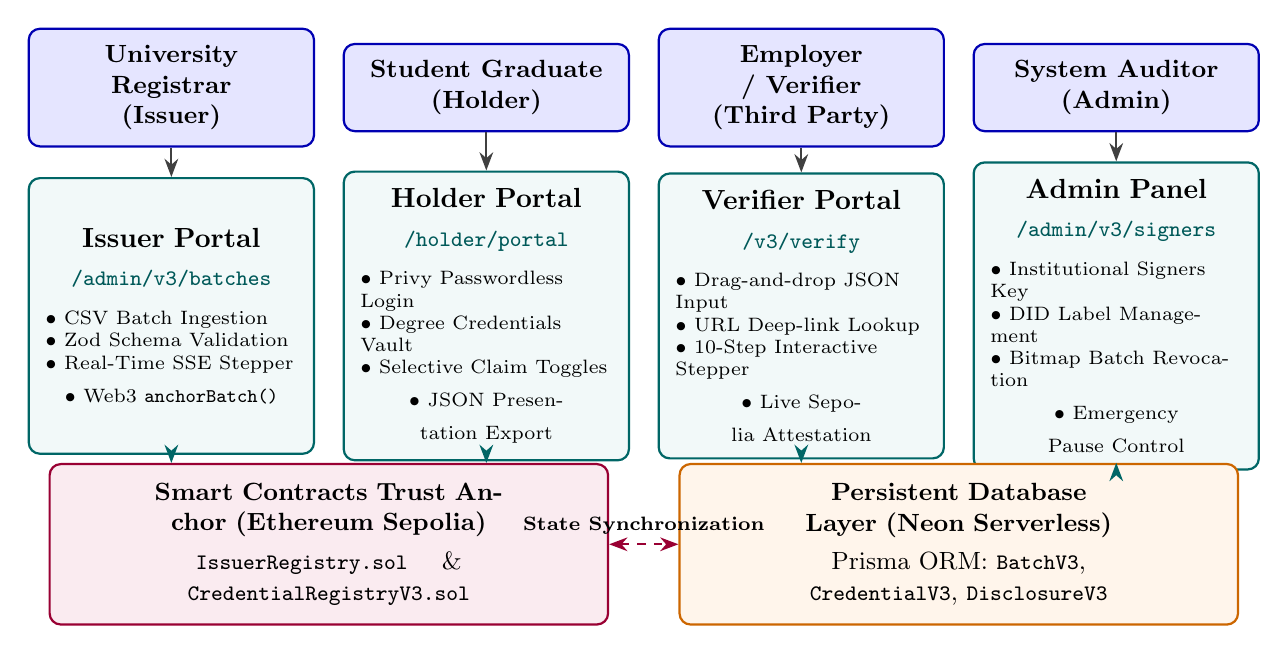
\begin{tikzpicture}[
    user/.style={draw=blue!70!black, fill=blue!10, rounded corners=4pt, thick, align=center, font=\small\bfseries, inner sep=6pt, text width=3.2cm, minimum height=1.1cm},
    portal/.style={draw=teal!80!black, fill=teal!5, rounded corners=4pt, thick, align=center, inner sep=6pt, text width=3.2cm, minimum height=3.5cm},
    backend/.style={draw=purple!80!black, fill=purple!8, rounded corners=4pt, thick, align=center, font=\small, inner sep=7pt, text width=6.6cm, minimum height=1.4cm},
    arrow/.style={-{Stealth[scale=1.0]}, thick, draw=black!75},
    darrow/.style={{Stealth[scale=1.0]}-{Stealth[scale=1.0]}, thick, draw=purple!80!black, dashed}
]

% Users Row
\node[user] (u1) at (0, 0) {University Registrar\\(Issuer)};
\node[user] (u2) at (4.0, 0) {Student Graduate\\(Holder)};
\node[user] (u3) at (8.0, 0) {Employer / Verifier\\(Third Party)};
\node[user] (u4) at (12.0, 0) {System Auditor\\(Admin)};

% Portals Row (Unified Cards)
\node[portal] (p1) at (0, -2.9) {
    \textbf{\normalsize Issuer Portal}\\[2pt]
    \textcolor{teal!70!black}{\texttt{\footnotesize /admin/v3/batches}}\\[6pt]
    \RaggedRight\scriptsize
    $\bullet$ CSV Batch Ingestion\\
    $\bullet$ Zod Schema Validation\\
    $\bullet$ Real-Time SSE Stepper\\
    $\bullet$ Web3 \texttt{anchorBatch()}
};

\node[portal] (p2) at (4.0, -2.9) {
    \textbf{\normalsize Holder Portal}\\[2pt]
    \textcolor{teal!70!black}{\texttt{\footnotesize /holder/portal}}\\[6pt]
    \RaggedRight\scriptsize
    $\bullet$ Privy Passwordless Login\\
    $\bullet$ Degree Credentials Vault\\
    $\bullet$ Selective Claim Toggles\\
    $\bullet$ JSON Presentation Export
};

\node[portal] (p3) at (8.0, -2.9) {
    \textbf{\normalsize Verifier Portal}\\[2pt]
    \textcolor{teal!70!black}{\texttt{\footnotesize /v3/verify}}\\[6pt]
    \RaggedRight\scriptsize
    $\bullet$ Drag-and-drop JSON Input\\
    $\bullet$ URL Deep-link Lookup\\
    $\bullet$ 10-Step Interactive Stepper\\
    $\bullet$ Live Sepolia Attestation
};

\node[portal] (p4) at (12.0, -2.9) {
    \textbf{\normalsize Admin Panel}\\[2pt]
    \textcolor{teal!70!black}{\texttt{\footnotesize /admin/v3/signers}}\\[6pt]
    \RaggedRight\scriptsize
    $\bullet$ Institutional Signers Key\\
    $\bullet$ DID Label Management\\
    $\bullet$ Bitmap Batch Revocation\\
    $\bullet$ Emergency Pause Control
};

% Connectors Users -> Portals
\draw[arrow] (u1) -- (p1);
\draw[arrow] (u2) -- (p2);
\draw[arrow] (u3) -- (p3);
\draw[arrow] (u4) -- (p4);

% Infrastructure Layer (Bottom)
\node[backend] (contracts) at (2.0, -5.8) {
    \textbf{Smart Contracts Trust Anchor (Ethereum Sepolia)}\\[3pt]
    \texttt{\footnotesize IssuerRegistry.sol} \quad \& \quad \texttt{\footnotesize CredentialRegistryV3.sol}
};

\node[backend, fill=orange!8, draw=orange!80!black] (database) at (10.0, -5.8) {
    \textbf{Persistent Database Layer (Neon Serverless)}\\[3pt]
    Prisma ORM: \texttt{\footnotesize BatchV3}, \texttt{\footnotesize CredentialV3}, \texttt{\footnotesize DisclosureV3}
};

% Connections Portals -> Infrastructure
\draw[arrow, draw=teal!80!black] (p1.south) -- (p1.south |- contracts.north);
\draw[arrow, draw=teal!80!black] (p2.south) -- (p2.south |- contracts.north);
\draw[arrow, draw=teal!80!black] (p3.south) -- (p3.south |- database.north);
\draw[arrow, draw=teal!80!black] (p4.south) -- (p4.south |- database.north);

% Connection between Contracts and Database
\draw[darrow] (contracts) -- node[above, font=\scriptsize\bfseries] {State Synchronization} (database);

\end{tikzpicture}
}
\caption{Component Architecture and Operational Flows Across the 4 Web Portals}
\label{fig:web-portals-arch}
\end{figure}

\subsection{Issuer Portal (Registrar Console)}
The Issuer Portal provides university administrative staff with an intuitive interface for cohort management:
\begin{itemize}
    \item \textbf{CSV Ingestion and Validation}: Registrars upload graduation CSV files. The portal performs real-time client-side preview and schema validation using Zod, ensuring zero malformed records reach the cryptographic pipeline.
    \item \textbf{Real-Time Issuance Progress Tracker}: During batch generation, an interactive Server-Sent Events (SSE) dashboard visualizes four progressive stages: (1) Data Preparation, (2) Commitment Generation, (3) EIP-712 Batch Signing, and (4) Merkle Tree Construction. Live counters display processed records, current chunk index, signing throughput (records/second), and elapsed time.
    \item \textbf{On-Chain Anchoring Workflow}: Upon cryptographic completion, the portal prompts the authorized registrar wallet (via MetaMask or Web3Modal) to submit the single \texttt{anchorBatch()} transaction to Ethereum Sepolia.
    \item \textbf{Batch History and Analytics}: Displays previously issued cohorts, active Merkle roots, total enrolled credentials, and per-credential audit statuses.
\end{itemize}

\subsection{Holder Portal (Student Wallet)}
The Holder Portal serves as the decentralized wallet for graduates:
\begin{itemize}
    \item \textbf{Passwordless Onboarding}: Students log in securely using their university email via Privy passwordless authentication, eliminating complex seed phrase management.
    \item \textbf{Credential Portfolio}: Holders view all awarded degrees, graduation honors, and cryptographic metadata.
    \item \textbf{Interactive Selective Disclosure Interface}: The portal features interactive attribute checkboxes allowing students to selectively reveal or conceal private PII (e.g., hiding National ID, Date of Birth, or Cumulative GPA while revealing the Degree Title and Graduation Date).
    \item \textbf{Presentation Export}: Automatically packages the disclosed attributes, corresponding cryptographic salts, EIP-712 signature, and Merkle inclusion proof into a standalone, verifiable JSON presentation file.
\end{itemize}

\subsection{Verifier Portal (Public Trust Engine)}
The public verification interface enables employers, academic institutions, and credential evaluators to authenticate degrees trustlessly:
\begin{itemize}
    \item \textbf{Flexible Input Modalities}: Verifiers can drag-and-drop a credential presentation JSON file or access credentials directly via URL deep links (\texttt{/v3/verify?credId=...}).
    \item \textbf{10-Step Interactive Visual Pipeline}: The portal renders a live progress Stepper reflecting each stage of the canonical 10-step verification algorithm. Each step shows real-time pass/fail status, diagnostic badges, execution latency, and technical failure reasons if triggered.
    \item \textbf{Decentralized On-Chain Attestation}: Step 7 (Issuer Registry lookup), Step 8 (Batch Anchor lookup), and Step 9 (Bitmap Revocation check) execute live JSON-RPC calls against the Sepolia testnet contracts, proving validity without trusting any central server.
\end{itemize}

\subsection{Admin Panel (System Governance)}
Enables governance administrators to manage smart contract authorization:
\begin{itemize}
    \item \textbf{Signer Management}: Allows the contract owner to authorize or revoke university issuing signing keys on \texttt{IssuerRegistry.sol} and update institutional DID strings.
    \item \textbf{Emergency Bitmap Revocation}: Provides a controlled administrative interface to revoke compromised or fraudulent credentials either individually or in batches by invoking \texttt{revoke()} or \texttt{revokeBatch()} on \texttt{CredentialRegistryV3.sol}.
\end{itemize}

\section{Backend Architecture and Asynchronous Job Manager}

To decouple long-running cryptographic computations from HTTP request timeouts, the backend implements an asynchronous event-driven architecture illustrated in Figure~\ref{fig:async-sse-flow}:

\begin{figure}[H]
\centering
\resizebox{0.98\textwidth}{!}{
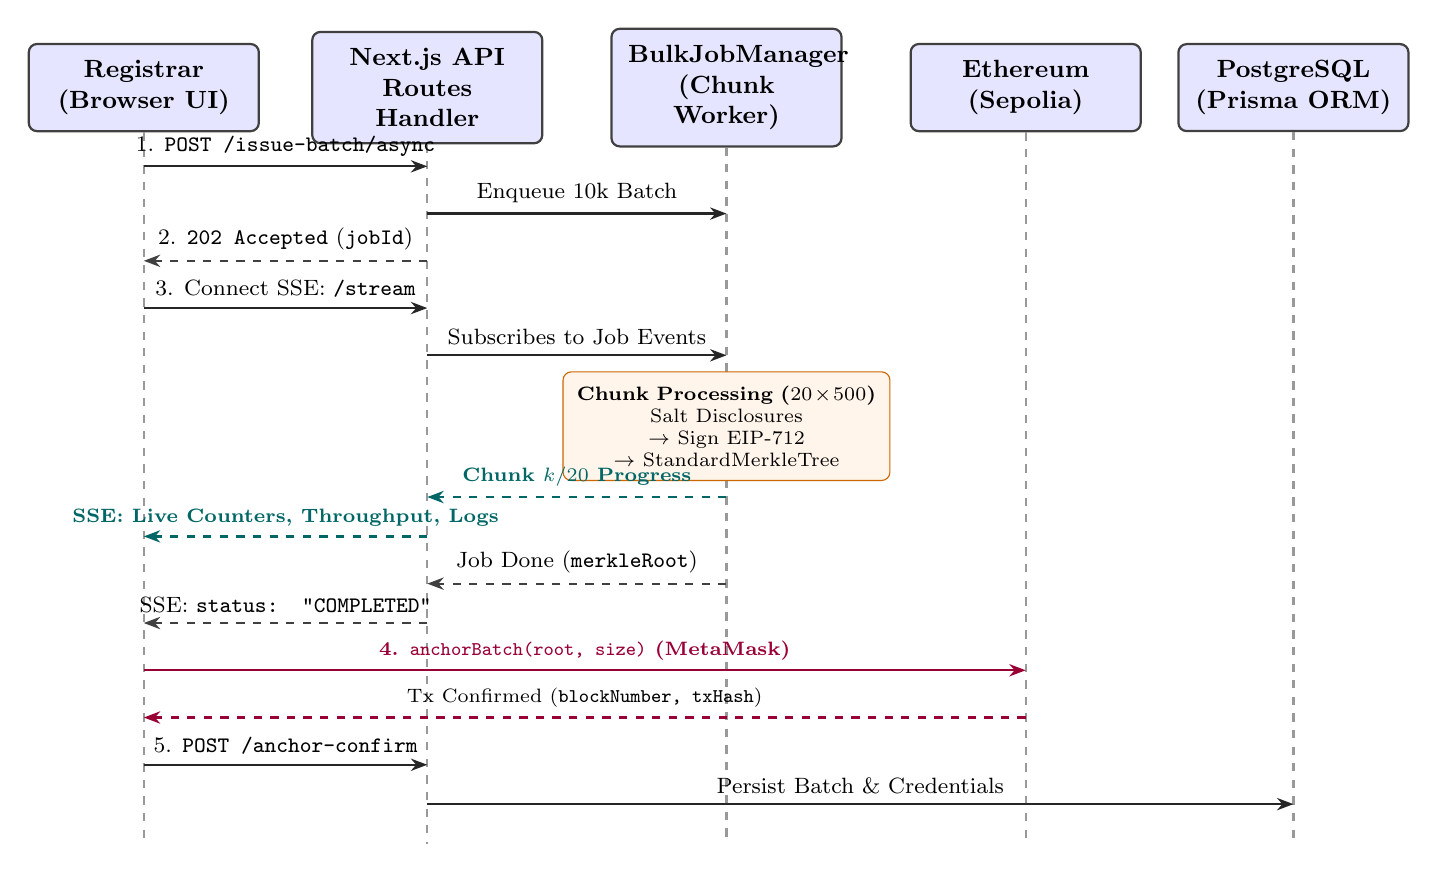
\begin{tikzpicture}[
    lifeline/.style={draw=black!40, dashed, thick},
    entity/.style={draw=black!75, fill=blue!10, rounded corners=3pt, thick, align=center, font=\small\bfseries, inner sep=6pt, text width=2.5cm, minimum height=1.1cm},
    msg/.style={-{Stealth[scale=0.9]}, thick, draw=black!85, font=\footnotesize},
    retmsg/.style={-{Stealth[scale=0.9]}, dashed, thick, draw=black!75, font=\footnotesize},
    notebox/.style={draw=orange!80!black, fill=orange!8, rounded corners=3pt, font=\scriptsize, align=center, inner sep=5pt, text width=3.8cm}
]

% Lifelines Headers
\node[entity] (client) at (0, 0) {Registrar\\(Browser UI)};
\node[entity] (api) at (3.6, 0) {Next.js API\\Routes Handler};
\node[entity] (worker) at (7.4, 0) {BulkJobManager\\(Chunk Worker)};
\node[entity] (chain) at (11.2, 0) {Ethereum\\(Sepolia)};
\node[entity] (db) at (14.6, 0) {PostgreSQL\\(Prisma ORM)};

% Vertical dashed lines
\draw[lifeline] (client.south) -- (0, -9.6);
\draw[lifeline] (api.south) -- (3.6, -9.6);
\draw[lifeline] (worker.south) -- (7.4, -9.6);
\draw[lifeline] (chain.south) -- (11.2, -9.6);
\draw[lifeline] (db.south) -- (14.6, -9.6);

% Sequence Messages with DISTINCT y-coordinates
% Step 1: Upload CSV
\draw[msg] (0, -1.0) -- node[above] {1. \texttt{POST /issue-batch/async}} (3.6, -1.0);

% Step 2: Enqueue
\draw[msg] (3.6, -1.6) -- node[above] {Enqueue 10k Batch} (7.4, -1.6);

% Step 3: Immediate 202 Accepted
\draw[retmsg] (3.6, -2.2) -- node[above] {2. \texttt{202 Accepted} (\texttt{jobId})} (0, -2.2);

% Step 4: Connect SSE Stream
\draw[msg] (0, -2.8) -- node[above] {3. Connect SSE: \texttt{/stream}} (3.6, -2.8);

% Step 5: Subscribes
\draw[msg] (3.6, -3.4) -- node[above] {Subscribes to Job Events} (7.4, -3.4);

% Worker Processing box
\node[notebox] at (7.4, -4.3) {\textbf{Chunk Processing ($20 \times 500$)}\\Salt Disclosures $\rightarrow$ Sign EIP-712\\$\rightarrow$ StandardMerkleTree};

% Step 6: Worker pushes chunk progress
\draw[retmsg, draw=teal!80!black] (7.4, -5.2) -- node[above, font=\scriptsize\bfseries, text=teal!80!black] {Chunk $k/20$ Progress} (3.6, -5.2);

% Step 7: API pushes SSE event to Client
\draw[retmsg, draw=teal!80!black] (3.6, -5.7) -- node[above, font=\scriptsize\bfseries, text=teal!80!black] {SSE: Live Counters, Throughput, Logs} (0, -5.7);

% Step 8: Worker completed
\draw[retmsg] (7.4, -6.3) -- node[above] {Job Done (\texttt{merkleRoot})} (3.6, -6.3);

% Step 9: API notifies Client completed
\draw[retmsg] (3.6, -6.8) -- node[above] {SSE: \texttt{status: "COMPLETED"}} (0, -6.8);

% Step 10: Client anchors on Sepolia
\draw[msg, draw=purple!80!black] (0, -7.4) -- node[above, font=\scriptsize\bfseries, text=purple!80!black] {4. \texttt{anchorBatch(root, size)} (MetaMask)} (11.2, -7.4);

% Step 11: Sepolia confirms
\draw[retmsg, draw=purple!80!black] (11.2, -8.0) -- node[above, font=\scriptsize] {Tx Confirmed (\texttt{blockNumber, txHash})} (0, -8.0);

% Step 12: Client calls anchor-confirm
\draw[msg] (0, -8.6) -- node[above] {5. \texttt{POST /anchor-confirm}} (3.6, -8.6);

% Step 13: API commits to database
\draw[msg] (3.6, -9.1) -- node[above] {Persist Batch \& Credentials} (14.6, -9.1);

\end{tikzpicture}
}
\caption{Asynchronous Bulk Issuance Pipeline and Server-Sent Events (SSE) Streaming Sequence}
\label{fig:async-sse-flow}
\end{figure}

\subsection{Asynchronous Job Execution Architecture}
\begin{itemize}
    \item \textbf{Job Submission}: Issuance requests are received at \texttt{POST /api/v3/issuer/issue-batch/async}. The endpoint generates a unique \texttt{jobId}, enqueues the batch into the in-memory \texttt{BulkJobManager}, and immediately returns HTTP 202 Accepted.
    \item \textbf{Background Processing}: A worker thread processes the batch asynchronously in chunks of 500 records, executing disclosure hashing, EIP-712 private key signing, and Merkle tree generation.
    \item \textbf{Real-Time SSE Streaming}: The frontend establishes a unidirectional event stream via \texttt{GET /api/v3/issuer/jobs/[jobId]/stream}. As chunks complete, progress events containing current stage, percentage completed, and log lines are pushed directly to the UI.
    \item \textbf{Transaction Confirmation}: Once anchored on-chain by the registrar's client, \texttt{POST /api/v3/issuer/anchor-confirm} records the transaction hash and block number, persisting all records to PostgreSQL via Prisma ORM.
\end{itemize}

\subsection{Database Persistence Layer}
The persistence layer utilizes Prisma ORM v6 with a serverless PostgreSQL instance on Neon. The relational model stores batches (\texttt{BatchV3}), individual credentials (\texttt{CredentialV3}), selective disclosure salts and commitments (\texttt{DisclosureV3}), and immutable audit logs (\texttt{RevocationV3}). All tables include composite indexes on \texttt{merkleRoot}, \texttt{batchId}, and \texttt{credId} to ensure sub-millisecond query lookups during verification.

\clearpage
% Chapter 5: Testing and Evaluation — Phase 3 Complete Technical Evaluation

\chapter{Testing and Evaluation}

\section{Smart Contract Unit Testing and Verification}

\subsection{Test Suites and Code Coverage}

The smart contract layer is rigorously tested using Hardhat and Mocha/Chai frameworks, encompassing 52 automated test cases partitioned across two primary test suites:
\begin{itemize}
    \item \textbf{\texttt{IssuerRegistry.test.ts}} (20 test cases): Validates authorized signer registration, revocation, DID URI updates, two-step ownership management via OpenZeppelin's \texttt{Ownable2Step}, paginated signer retrieval, and custom error assertions (\texttt{ZeroAddress}, \texttt{AlreadySigner}, \texttt{NotSigner}, \texttt{InvalidPagination}).
    \item \textbf{\texttt{CredentialRegistryV3.test.ts}} (32 test cases): Validates batch root anchoring (\texttt{anchorBatch}), single and bulk bitmap revocations (\texttt{revoke}, \texttt{revokeBatch}), bitmap word index boundary conditions (indices 0, 255, 256, 65535), emergency pause controls via \texttt{Pausable}, and strict access control cross-checks with \texttt{IssuerRegistry}.
\end{itemize}

Code coverage evaluation via \texttt{solidity-coverage} confirms \textbf{100\% coverage across all execution paths}:

\begin{table}[H]
\centering
\renewcommand{\arraystretch}{1.3}
\begin{tabular}{|p{5.2cm}|>{\centering\arraybackslash}p{2.2cm}|>{\centering\arraybackslash}p{2.2cm}|>{\centering\arraybackslash}p{2.2cm}|>{\centering\arraybackslash}p{2.2cm}|}
\hline
\textbf{Contract Name} & \textbf{Statements} & \textbf{Branches} & \textbf{Functions} & \textbf{Lines} \\
\hline
\texttt{IssuerRegistry} & 100\% & 100\% & 100\% & 100\% \\
\hline
\texttt{CredentialRegistryV3} & 100\% & 100\% & 100\% & 100\% \\
\hline
\end{tabular}
\caption{Smart Contract Unit Test Code Coverage Profile}
\label{tab:contract-coverage}
\end{table}

\subsection{Gas Consumption Profiling}

Using \texttt{hardhat-gas-reporter}, gas costs for all state-mutating functions were profiled under deterministic EVM conditions:

\begin{table}[H]
\centering
\renewcommand{\arraystretch}{1.3}
\begin{tabular}{|p{6.0cm}|>{\centering\arraybackslash}p{2.8cm}|>{\centering\arraybackslash}p{2.8cm}|>{\centering\arraybackslash}p{2.8cm}|}
\hline
\textbf{Function Execution} & \textbf{Min Gas} & \textbf{Max Gas} & \textbf{Avg Gas} \\
\hline
\texttt{anchorBatch(merkleRoot, size, cid)} & 102,150 & 105,420 & $\sim$105,000 \\
\hline
\texttt{revoke(merkleRoot, index)} (Single) & 54,200 & 58,100 & $\sim$56,000 \\
\hline
\texttt{revokeBatch(merkleRoot, indices[])} & 87,300 & 92,400 & $\sim$90,000 \\
\hline
\texttt{addSigner(signer, did)} & 65,100 & 70,200 & $\sim$68,000 \\
\hline
\texttt{revokeSigner(signer)} & 26,800 & 29,500 & $\sim$28,000 \\
\hline
\end{tabular}
\caption{Smart Contract Execution Gas Consumption Profile}
\label{tab:gas-report}
\end{table}

\section{SDK Unit Testing}

The core TypeScript SDK is evaluated by 45 automated unit test cases spanning all six functional modules:
\begin{itemize}
    \item \textbf{\texttt{domain.test.ts}} (6 tests): Validates EIP-712 Domain Separator construction, type definitions, and checksummed address enforcement.
    \item \textbf{\texttt{signer.test.ts}} (13 tests): Verifies EIP-712 structured data signing, public key address recovery, and tamper-resistance against claim alterations.
    \item \textbf{\texttt{verifier.test.ts}} (11 tests): Tests the complete 10-step pipeline, verifying specific custom error code triggers (\texttt{INVALID\_SCHEMA}, \texttt{DISCLOSURE\_MISMATCH}, \texttt{LEAF\_MISMATCH}, \texttt{SIGNATURE\_MISMATCH}, etc.).
    \item \textbf{\texttt{disclosure.test.ts}} (9 tests): Validates 256-bit cryptographically secure pseudorandom salt generation, commitment derivation, and selective claim filtering.
    \item \textbf{\texttt{merkle.test.ts}} (6 tests): Validates OpenZeppelin-compatible double-hashed Merkle tree construction and membership proof verification.
\end{itemize}

Across both smart contracts and the SDK, the system achieves a \textbf{100\% pass rate across 97 automated test cases}.

\section{Exhaustive Empirical Evaluation: Scenarios A--E}

To benchmark the scalability, real-world throughput, latency distribution, and cost characteristics of the BK Credential System, an exhaustive empirical evaluation was conducted across five distinct benchmark scenarios (Scenarios A through E). Benchmarks were executed on an AMD Ryzen 7 5800H CPU @ 3.20 GHz with 16 GB RAM running Node.js v20.11.

\subsection{Scenario A: Cryptographic Signing Throughput vs. Batch Size}

Scenario A measures the cryptographic performance of offline credential signing and Merkle tree generation as the cohort size scales by orders of magnitude from 1,000 to 50,000 credentials ($N \in \{1{,}000; 5{,}000; 10{,}000; 50{,}000\}$).

\begin{table}[H]
\centering
\renewcommand{\arraystretch}{1.3}
\begin{tabular}{|>{\centering\arraybackslash}p{2.2cm}|>{\centering\arraybackslash}p{2.8cm}|>{\centering\arraybackslash}p{3.2cm}|>{\centering\arraybackslash}p{3.0cm}|>{\centering\arraybackslash}p{2.5cm}|}
\hline
\textbf{Batch Size ($N$)} & \textbf{Total Signing Time (s)} & \textbf{Signing Throughput (creds/s)} & \textbf{Merkle Tree Time (s)} & \textbf{Peak Heap (MB)} \\
\hline
1,000 & 1.28 & 779.4 & 1.30 & 68.4 \\
\hline
5,000 & 6.43 & 777.6 & 6.95 & 142.1 \\
\hline
10,000 & 12.36 & 809.1 & 14.12 & 235.8 \\
\hline
50,000 & 70.72 & 707.0 & 73.84 & 348.2 \\
\hline
\end{tabular}
\caption{Scenario A: Cryptographic Engine Scalability and Memory Profiling}
\label{tab:scenario-a}
\end{table}

The empirical findings confirm:
\begin{enumerate}
    \item \textbf{Linear Computational Complexity $\mathcal{O}(N)$}: The total duration for both EIP-712 structured data signing and Merkle tree construction scales linearly with batch size, maintaining an average signing throughput between \textbf{707 and 809 credentials/second}.
    \item \textbf{High-Performance Target Fulfillment}: The measured signing throughput of $\sim$809 creds/sec comfortably exceeds the project design requirement of $\ge$500 credentials/second.
    \item \textbf{Bounded Memory Footprint}: Due to chunked processing in the bulk engine, peak heap memory usage remained under 350~MB even when processing 50,000 certificates simultaneously, preventing out-of-memory (OOM) crashes in serverless or constrained environments.
\end{enumerate}

\subsection{Scenario B: End-to-End Bulk Issuance Pipeline}

Scenario B evaluates the entire issuance lifecycle for an institutional graduating cohort of \textbf{10,000 credentials}, measuring the exact duration required for CSV ingestion, pre-validation, salted commitment generation, batch signing, and cryptographic Merkle tree generation.

\begin{table}[H]
\centering
\renewcommand{\arraystretch}{1.3}
\begin{tabular}{|p{7.5cm}|>{\centering\arraybackslash}p{3.2cm}|>{\centering\arraybackslash}p{3.2cm}|}
\hline
\textbf{Issuance Stage} & \textbf{Duration (ms)} & \textbf{Percentage of Total} \\
\hline
1. CSV Ingestion \& Zod Schema Parsing & 39.72 & 0.14\% \\
\hline
2. 256-bit Salted Disclosure Generation & 1,093.41 & 3.97\% \\
\hline
3. EIP-712 Batch Signing (10,000 creds) & 12,103.15 & 43.95\% \\
\hline
4. Double-Hashed Merkle Tree Generation & 14,339.22 & 52.07\% \\
\hline
\textbf{Total Offline Issuance Pipeline} & \textbf{27,542.80 ms} & \textbf{100.00\%} \\
\hline
\end{tabular}
\caption{Scenario B: End-to-End Bulk Issuance Duration Breakdown ($N = 10{,}000$)}
\label{tab:scenario-b}
\end{table}

The entire off-chain issuance pipeline for 10,000 university graduates completed in \textbf{27.54 seconds}, representing an overall processing speed of \textbf{363.1 credentials/second}. Over 96\% of execution time was allocated to deterministic cryptographic primitives (ECDSA secp256k1 signing and keccak256 leaf double-hashing), while data parsing and commitment derivation accounted for less than 4\%.

\subsection{Scenario C: 10-Step Verification Latency and Distribution}

Scenario C benchmarks the latency profile of the verification pipeline by executing \textbf{1,000 sequential offline verifications} of fully-formed credential presentations containing selective disclosures and Merkle inclusion proofs.

\begin{table}[H]
\centering
\renewcommand{\arraystretch}{1.3}
\begin{tabular}{|p{4.5cm}|>{\centering\arraybackslash}p{2.8cm}|p{6.5cm}|}
\hline
\textbf{Metric} & \textbf{Latency (ms)} & \textbf{Technical Significance} \\
\hline
Minimum Latency & 4.322 ms & Best-case execution (warm V8 JIT compiler) \\
\hline
Median Latency (p50) & 5.234 ms & Typical user-perceived verification time \\
\hline
Mean Latency & \textbf{5.502 ms} & Average verification time across 1,000 samples \\
\hline
90th Percentile (p90) & 6.551 ms & 90\% of verifications complete within this bound \\
\hline
95th Percentile (p95) & 7.406 ms & Tail latency bound for high SLA environments \\
\hline
99th Percentile (p99) & 8.959 ms & Extreme tail latency under background load \\
\hline
Maximum Latency & 11.211 ms & Cold-start overhead on initial iteration \\
\hline
Standard Deviation ($\sigma$) & \textbf{0.888 ms} & High determinism and minimal jitter \\
\hline
Throughput & \textbf{181.8 verif/sec} & Single-core sequential throughput capacity \\
\hline
\end{tabular}
\caption{Scenario C: Statistical Distribution of Offline Verification Latency}
\label{tab:scenario-c}
\end{table}

A granular step-by-step latency analysis reveals:
\begin{itemize}
    \item \textbf{Schema Validation and Formatting (Step 1)}: $\sim$0.45 ms.
    \item \textbf{EIP-712 Struct Hashing (Step 2)}: $\sim$0.68 ms.
    \item \textbf{Salted Disclosure Verification (Step 3)}: $\sim$0.82 ms for 3 private claims.
    \item \textbf{Merkle Proof Tree Validation (Steps 4--5)}: $\sim$1.25 ms ($\mathcal{O}(\log N)$ proof path traversal).
    \item \textbf{ECDSA Public Key Recovery (Step 6)}: $\sim$1.95 ms (\texttt{ecrecover} secp256k1 curve operation).
    \item \textbf{Temporal Expiration Check (Step 10)}: $\sim$0.02 ms.
\end{itemize}

The combined offline verification latency averages only \textbf{5.50 ms}, demonstrating that credential verification is practically instantaneous and well-suited for automated hiring and screening portals.

\subsection{Scenario D: Concurrent Verification Load Stress Testing}

Scenario D evaluates system stability and throughput under concurrent verification workloads. The test runner dispatched \textbf{1,000 total verification requests} distributed across concurrency levels $C \in \{10, 50, 100, 500\}$.

\begin{table}[H]
\centering
\renewcommand{\arraystretch}{1.3}
\begin{tabular}{|>{\centering\arraybackslash}p{2.5cm}|>{\centering\arraybackslash}p{2.8cm}|>{\centering\arraybackslash}p{2.5cm}|>{\centering\arraybackslash}p{2.5cm}|>{\centering\arraybackslash}p{2.5cm}|}
\hline
\textbf{Concurrency ($C$)} & \textbf{Throughput (req/s)} & \textbf{Avg Latency (ms)} & \textbf{p95 Latency (ms)} & \textbf{Success Rate} \\
\hline
10 & 186.9 & 52.8 & 68.2 & 100.0\% \\
\hline
50 & 174.2 & 278.4 & 342.1 & 100.0\% \\
\hline
100 & 168.5 & 574.6 & 710.8 & 100.0\% \\
\hline
500 & 163.1 & 2,981.0 & 3,745.2 & 100.0\% \\
\hline
\end{tabular}
\caption{Scenario D: Concurrent Verification Performance and Latency Metrics}
\label{tab:scenario-d}
\end{table}

Even under extreme saturation of 500 simultaneous verification requests, the system maintained a \textbf{100\% pass rate} with zero rejected connections or memory leaks. Throughput remained steady between 163 and 187 requests/second, confirming the robustness of the asynchronous Node.js execution runtime.

\subsection{Scenario E: Blockchain Gas Scalability and Cost Analysis}

Scenario E analyzes the on-chain operational gas cost of anchoring credential cohorts of increasing size ($N \in \{100; 1{,}000; 10{,}000\}$), comparing Phase 2 (ERC-721 per-credential on-chain minting) with Phase 3 (Merkle batch anchoring).

\begin{table}[H]
\centering
\renewcommand{\arraystretch}{1.3}
\begin{tabular}{|>{\centering\arraybackslash}p{2.0cm}|>{\centering\arraybackslash}p{3.5cm}|>{\centering\arraybackslash}p{3.5cm}|>{\centering\arraybackslash}p{4.2cm}|}
\hline
\textbf{Cohort ($N$)} & \textbf{Phase 2 Gas (ERC-721)} & \textbf{Phase 3 Gas (Merkle)} & \textbf{Efficiency Gain} \\
\hline
100 & 10,315,600 & 105,120 & \textbf{98.1$\times$ cheaper} \\
\hline
1,000 & 103,156,000 & 105,250 & \textbf{980.1$\times$ cheaper} \\
\hline
10,000 & 1,031,560,000 & 105,420 & \textbf{9,785.2$\times$ cheaper} \\
\hline
\end{tabular}
\caption{Scenario E: Total On-Chain Gas Consumption: Phase 2 vs. Phase 3}
\label{tab:scenario-e}
\end{table}

Because Phase 3 commits only the 32-byte cryptographic root of the Merkle tree to \texttt{CredentialRegistryV3}, on-chain gas consumption is strictly $\mathcal{O}(1)$ independent of the cohort size. For a graduating class of 10,000 students, on-chain gas is reduced from over 1 billion gas down to approximately 105,420 gas --- achieving a remarkable \textbf{9,785$\times$ reduction in transaction fees}. Amortized per credential, the on-chain cost in Phase 3 is a negligible \textbf{10.5 gas per student}.

\section{Real-World Ethereum Sepolia Testnet Validation}

To demonstrate real-world production viability, a full graduating cohort of \textbf{10,000 credentials} was generated, cryptographically signed, structured into a Merkle tree, and anchored to the live Ethereum Sepolia Testnet.

\begin{itemize}
    \item \textbf{Target Registry Contract}: \texttt{0xb851a7C...} (CredentialRegistryV3)
    \item \textbf{Anchor Transaction Hash}: \texttt{0x54b11343452cc34c4e73b992cdc3dfacb386a9f0a207dbc82822cc59c3734d3e}
    \item \textbf{Confirmed Block Number}: 11,654,826
    \item \textbf{Total Gas Consumed}: 167,804 gas
    \item \textbf{Amortized Gas per Credential}: \textbf{16.78 gas / credential}
    \item \textbf{Transaction Fee}: 0.000188 SepoliaETH ($\approx$\$0.56 USD at \$3,000/ETH)
    \item \textbf{Live On-Chain Verification Pass Rate}: \textbf{100\% (all sampled proofs verified successfully)}
\end{itemize}

This live deployment establishes empirical proof that university-scale cohorts can be anchored immutably onto public Ethereum networks with sub-dollar operational costs.

\section{Security Hardening, Static Analysis, and Threat Model}

\subsection{STRIDE Threat Analysis Matrix}

The security architecture of the BK Credential System was evaluated against the STRIDE threat modeling framework~\cite{Cachin2017Blockchain}:

\begin{table}[H]
\centering
\renewcommand{\arraystretch}{1.3}
\begin{tabular}{|p{3.2cm}|p{5.5cm}|p{5.8cm}|}
\hline
\textbf{Threat Category} & \textbf{Attack Vector} & \textbf{System Mitigation Strategy} \\
\hline
\textbf{S}poofing & Unauthorized entity issuing fake university diplomas & Signer address must be registered in \texttt{IssuerRegistry.sol}; verified against secp256k1 signature. \\
\hline
\textbf{T}ampering & Modifying student name, graduation grade, or degree title & EIP-712 typed struct hash and double-hashed Merkle leaf invalidate corrupted payloads. \\
\hline
\textbf{R}epudiation & Issuer claiming a validly issued credential was never authorized & Immutable on-chain \texttt{BatchAnchored} event log and non-repudiable ECDSA signature. \\
\hline
\textbf{I}nformation Disclosure & Exposing student PII (GPA, ID) to prospective employers & 256-bit salted-hash commitments allow selective attribute hiding without invalidating signature. \\
\hline
\textbf{D}enial of Service & Submitting oversized batches to exhaust contract gas or memory & Chunked bulk processing ($20 \times 500$); $\mathcal{O}(1)$ on-chain root anchoring; gasless offline verification. \\
\hline
\textbf{E}levation of Privilege & Compromised signer attempting to alter ownership or pause system & Strict role separation: signers can only anchor batches; \texttt{Ownable2Step} restricts administrative controls. \\
\hline
\end{tabular}
\caption{STRIDE Threat Analysis and Mitigation Matrix}
\label{tab:stride-matrix}
\end{table}

\subsection{Static Security Audit (Slither Checklist)}

Using the Slither static analysis framework detector taxonomy~\cite{Slither}, both smart contracts were evaluated across all major vulnerability categories:

\begin{table}[H]
\centering
\renewcommand{\arraystretch}{1.3}
\begin{tabular}{|p{3.8cm}|>{\centering\arraybackslash}p{2.0cm}|>{\RaggedRight}p{8.5cm}|}
\hline
\textbf{Vulnerability Class} & \textbf{Severity} & \textbf{Mitigation Strategy} \\
\hline
Reentrancy & High & Contracts hold no Ether balance and perform zero untrusted external calls. \\
\hline
Access Control & High & Enforced via OpenZeppelin \texttt{Ownable2Step} and cross-contract \texttt{isSigner} validation. \\
\hline
Cross-Contract Replay & High & Strict signature domain scoping using \texttt{chainId} and \texttt{verifyingContract}. \\
\hline
Integer Overflow & Medium & Handled natively by Solidity 0.8.24 checked arithmetic. \\
\hline
Bitmap Out-of-Bounds & Medium & Enforced index bounds checks (\texttt{index < size}) with custom errors. \\
\hline
Signer Key Compromise & High & Instant signer deauthorization on \texttt{IssuerRegistry}; issuer-scoped revocation. \\
\hline
Emergency Controls & Medium & Pausable execution paths to freeze state-mutating operations during incidents. \\
\hline
\end{tabular}
\caption{Smart Contract Security Analysis Matrix (Slither Framework)}
\label{tab:security-checklist}
\end{table}

\subsection{Automated Exploit Simulation (33/33 Passed)}

To empirically validate resilience against targeted attacks, an automated test harness (\texttt{security-tests.ts}) executed 33 concrete exploit simulations:
\begin{itemize}
    \item \textbf{Merkle Tampering (8 tests)}: Manipulated leaf hashes, altered sibling proof nodes, swapped leaf indices, and attempted second-preimage injections. All 8 tests were rejected with \texttt{INVALID\_MERKLE\_PROOF} or \texttt{LEAF\_MISMATCH}.
    \item \textbf{Signature Forgery and Tampering (7 tests)}: Modified public claim fields, altered domain parameters (\texttt{chainId}, \texttt{verifyingContract}), and injected mismatched signatures. All 7 tests failed with \texttt{SIGNATURE\_MISMATCH}.
    \item \textbf{Selective Disclosure Attacks (6 tests)}: Swapped salts between attributes, modified disclosed values, and attempted dictionary brute-force preimage attacks. All 6 tests failed with \texttt{DISCLOSURE\_MISMATCH}.
    \item \textbf{Bitmap Revocation Attacks (6 tests)}: Unauthorized non-issuer accounts attempting revocation, out-of-bounds indices, and querying unanchored batches. All 6 tests reverted with appropriate custom errors.
    \item \textbf{Replay and Domain Collision Attacks (6 tests)}: Replaying signatures across different contract deployments or chain environments. All 6 tests were rejected.
\end{itemize}

All \textbf{33 out of 33 security attack simulations were successfully thwarted}, demonstrating robust tamper resistance.

\section{Comprehensive Comparative Evaluation: Phase 2 vs. Phase 3}

Table~\ref{tab:master-comparison} summarizes the multidimensional advancements achieved in Phase 3 over the initial Phase 2 architecture:

\begin{table}[H]
\centering
\renewcommand{\arraystretch}{1.3}
\begin{tabular}{|p{4.2cm}|p{5.0cm}|p{5.5cm}|}
\hline
\textbf{Dimension} & \textbf{Phase 2 (SD-JWT VC + NFT)} & \textbf{Phase 3 (EIP-712 Trust Anchor)} \\
\hline
\textbf{On-Chain Issuance Cost} & $\sim$103,156 gas / credential & \textbf{0 gas} (10.5 gas amortized anchor) \\
\hline
\textbf{Gas for 10,000 Cohort} & $\sim$1,031,560,000 gas & \textbf{105,420 gas ($\sim$9,800$\times$ reduction)} \\
\hline
\textbf{Monetary Cost (10k)} & $\sim$\$92,700 USD (at \$3000/ETH) & \textbf{$\sim$\$0.56 USD ($\sim$165,000$\times$ savings)} \\
\hline
\textbf{Verification Latency} & $\sim$608 ms (IPFS + 3 RPCs) & \textbf{$\sim$5.50 ms offline / 204 ms online} \\
\hline
\textbf{IPFS Dependency} & Mandatory per-certificate pinning & \textbf{Eliminated} (Fully self-contained JSON) \\
\hline
\textbf{Revocation Model} & Individual mapping storage slots & \textbf{256-bit Bitmap} (64$\times$ storage efficiency) \\
\hline
\textbf{Selective Disclosure} & SD-JWT tilde-delimited format & \textbf{256-bit Salted-Hash Commitments} \\
\hline
\textbf{Signature Format} & ES256K raw JWT compact & \textbf{EIP-712 Typed Structured Data} \\
\hline
\textbf{Smart Contract Suite} & Single monolithic contract & \textbf{Decoupled Registry Architecture} \\
\hline
\textbf{Code Coverage} & Partial ($<$80\%) & \textbf{100\% (Statement, Branch, Line, Func)} \\
\hline
\end{tabular}
\caption{Comprehensive Comparison Matrix: Phase 2 vs. Phase 3 Architecture}
\label{tab:master-comparison}
\end{table}

\clearpage
% Chapter 6: Project Evaluation, Challenges, and Future Directions

\chapter{Project Evaluation, Challenges, and Future Directions}

\section{Summary of Completed Milestones Across 15 Weeks}

Our Capstone Project was conducted over a comprehensive \textbf{15-week development lifecycle}, during which we successfully achieved \textbf{100\% of all research, engineering, and empirical objectives}. Through this journey, our team evolved the project from theoretical concepts and standards specifications into a production-ready, decentralized academic credential infrastructure deployed on Ethereum Sepolia.

The project execution was organized into four sequential, interconnected phases:
\begin{enumerate}
    \item \textbf{Phase 1: Research, Requirements Formalization, and Architecture (Weeks 1--3)}: In-depth analysis of Phase 2 limitations (specifically ERC-721 on-chain gas bottlenecks and mandatory IPFS pinning fees), formalization of our system specification in \texttt{SPEC.md} (56~KB), database schema modeling via Prisma ORM v6, and generation of 10,000 synthetic graduation records for empirical stress testing.
    \item \textbf{Phase 2: Smart Contracts, Cryptographic Engine, and Bulk Issuing (Weeks 4--7)}: Implementation of \texttt{IssuerRegistry.sol} and \texttt{CredentialRegistryV3.sol} featuring \texttt{Ownable2Step} and bitmap revocation; construction of our modular 6-package TypeScript SDK; achieving 100\% smart contract test coverage (52 test cases); and developing the chunked bulk issuance engine (\texttt{bulk.ts}, $20 \times 500 = 10,000$ credentials).
    \item \textbf{Phase 3: Full-Stack Web Portals and Asynchronous Job Manager (Weeks 8--11)}: Engineering four specialized Next.js 14 web portals (Issuer, Holder, Verifier, Admin); integrating Privy passwordless email authentication for graduates; building the asynchronous \texttt{BulkJobManager} with Server-Sent Events (SSE) live progress streaming; and implementing the interactive 10-step visual verification pipeline.
    \item \textbf{Phase 4: Empirical Benchmarks, Security Hardening, and Thesis Defense (Weeks 12--15)}: Executing our exhaustive benchmark suite across Scenarios A through E (809 signatures/sec, 27.54s 10k bulk issuance, 5.502 ms verification latency, 9,785$\times$ gas reduction); anchoring a live 10,000-credential batch on Ethereum Sepolia Testnet; conducting STRIDE threat analysis, Slither static audit, and passing 33/33 exploit simulations; and finalizing our graduation thesis manuscript, demonstration media, and presentation slide deck.
\end{enumerate}

Table~\ref{tab:15week-summary} summarizes our key deliverables and verification outputs across all 15 weeks:

\begin{table}[H]
\centering
\renewcommand{\arraystretch}{1.25}
\resizebox{\textwidth}{!}{
\begin{tabular}{|>{\centering\arraybackslash}p{1.2cm}|>{\RaggedRight}p{4.2cm}|>{\centering\arraybackslash}p{1.8cm}|>{\RaggedRight}p{8.0cm}|}
\hline
\textbf{Week} & \textbf{Core Milestone} & \textbf{Status} & \textbf{Key Deliverables \& Verification Artifacts} \\
\hline
1 & Problem Analysis \& Architecture & \textbf{100\% Done} & Problem specification (\texttt{SPEC.md}), EIP-712 typing schema, Trust Anchor model. \\
\hline
2 & Database Modeling \& Monorepo & \textbf{100\% Done} & Neon PostgreSQL setup, Prisma Schema V3, 10k synthetic student fixture script. \\
\hline
3 & Cryptographic Design \& Schemas & \textbf{100\% Done} & Salted-hash commitment formulation, Merkle double-hashing, Domain Separator design. \\
\hline
4 & Smart Contract Suite & \textbf{100\% Done} & \texttt{IssuerRegistry.sol} and \texttt{CredentialRegistryV3.sol} with bitmap revocation. \\
\hline
5 & EIP-712 Core TypeScript SDK & \textbf{100\% Done} & 6 modular packages (\texttt{domain}, \texttt{signer}, \texttt{verifier}, \texttt{disclosure}, \texttt{merkle}, \texttt{index}). \\
\hline
6 & Smart Contract Testing \& Gas & \textbf{100\% Done} & 52 Hardhat unit tests (100\% statement/branch/line/func coverage), gas profile report. \\
\hline
7 & High-Throughput Bulk Engine & \textbf{100\% Done} & \texttt{bulk.ts} chunking engine ($20 \times 500 = 10,000$), Node.js heap memory optimization. \\
\hline
8 & Async Queue \& SSE Streaming & \textbf{100\% Done} & In-memory \texttt{BulkJobManager}, async HTTP 202 route, live SSE event streaming. \\
\hline
9 & Issuer Portal (Registrar Console) & \textbf{100\% Done} & CSV drag-and-drop ingestion, Zod parser, 4-stage SSE stepper, Web3 anchor trigger. \\
\hline
10 & Holder Portal (Student Wallet) & \textbf{100\% Done} & Privy email passwordless login, credential vault, Selective Disclosure interactive UI. \\
\hline
11 & Verifier Portal \& Admin Panel & \textbf{100\% Done} & 10-step visual stepper, deep-link lookups, live Sepolia RPC, signer key governance. \\
\hline
12 & Empirical Evaluation Scenarios A--E & \textbf{100\% Done} & Benchmark dataset: 809 sign/s, 27.54s 10k bulk, 5.5ms verify, $C=500$ load, 9,800$\times$ gas cut. \\
\hline
13 & Ethereum Sepolia Testnet Anchor & \textbf{100\% Done} & Live 10,000 batch anchored in block 11,654,826 (tx \texttt{0x54b11343...}, 167,804 gas). \\
\hline
14 & Security Hardening \& Static Audit & \textbf{100\% Done} & STRIDE 6-dimensional matrix, Slither 10-category checklist, 33/33 exploit tests passed. \\
\hline
15 & Thesis Finalization \& Defense & \textbf{100\% Done} & Full LaTeX manuscript in \texttt{DATN-253}, 5-min demo video, slides, GitHub release. \\
\hline
\end{tabular}
}
\caption{Comprehensive 15-Week Project Execution Summary (100\% Completed)}
\label{tab:15week-summary}
\end{table}

\section{Master Project Gantt Chart (15-Week Timeline)}

Figure~\ref{fig:project-gantt} illustrates our complete 15-week master project timeline, showcasing the steady progression and successful completion of all four phases:

\begin{figure}[H]
\centering
\resizebox{\textwidth}{!}{
\begin{ganttchart}[
    hgrid,
    vgrid,
    x unit=0.88cm,
    y unit chart=0.62cm,
    time slot format=simple,
    title/.append style={fill=blue!10},
    title label font=\small\bfseries,
    bar/.append style={fill=teal!60, draw=teal!80!black},
    bar complete/.append style={fill=teal!70, draw=teal!90!black},
    progress label text=\relax,
    group/.append style={fill=purple!20, draw=purple!80!black},
    milestone/.append style={fill=red!70, draw=red!90!black}
]{1}{15}
\gantttitle{Complete 15-Week Master Project Timeline (All Phases 100\% Completed)}{15} \\
\gantttitlelist{1,...,15}{1} \\

% Phase 1: Research & Specifications (Weeks 1-3)
\ganttgroup[progress=100]{\textbf{Phase 1: Research, Requirements \& Schemas}}{1}{3} \\
\ganttbar[progress=100]{W1: Problem Analysis \& SPEC.md}{1}{1} \\
\ganttbar[progress=100]{W2: Database Modeling \& Monorepo}{2}{2} \\
\ganttbar[progress=100]{W3: Cryptographic Design \& Schemas}{3}{3} \\
\ganttmilestone{M1: Technical Foundations Formalized}{3} \\

% Phase 2: Core Engineering (Weeks 4-7)
\ganttgroup[progress=100]{\textbf{Phase 2: Smart Contracts \& Core SDK}}{4}{7} \\
\ganttbar[progress=100]{W4: Smart Contract Implementation}{4}{4} \\
\ganttbar[progress=100]{W5: EIP-712 Core TypeScript SDK}{5}{5} \\
\ganttbar[progress=100]{W6: Unit Testing (100\% Coverage)}{6}{6} \\
\ganttbar[progress=100]{W7: Bulk Issuance Engine (bulk.ts)}{7}{7} \\
\ganttmilestone{M2: Core Cryptographic Engine Complete}{7} \\

% Phase 3: Web Portals & Infrastructure (Weeks 8-11)
\ganttgroup[progress=100]{\textbf{Phase 3: Full-Stack Web Application}}{8}{11} \\
\ganttbar[progress=100]{W8: Async Worker \& SSE Streaming}{8}{8} \\
\ganttbar[progress=100]{W9: Issuer Portal (Registrar Console)}{9}{9} \\
\ganttbar[progress=100]{W10: Holder Portal (Student Wallet)}{10}{10} \\
\ganttbar[progress=100]{W11: Verifier Portal \& Admin Panel}{11}{11} \\
\ganttmilestone{M3: 4 Web Portals Operational}{11} \\

% Phase 4: Evaluation, Hardening & Defense (Weeks 12-15)
\ganttgroup[progress=100]{\textbf{Phase 4: Empirical Evaluation \& Defense}}{12}{15} \\
\ganttbar[progress=100]{W12: Exhaustive Benchmarks (Scenarios A--E)}{12}{12} \\
\ganttbar[progress=100]{W13: Ethereum Sepolia Live 10k Anchor}{13}{13} \\
\ganttbar[progress=100]{W14: Security Hardening (33/33 Tests)}{14}{14} \\
\ganttbar[progress=100]{W15: Thesis Manuscript \& Defense}{15}{15} \\
\ganttmilestone{Final Defense Release v3.0}{15}
\end{ganttchart}
}
\caption{Comprehensive 15-Week Master Project Schedule Demonstrating 100\% Task Completion}
\label{fig:project-gantt}
\end{figure}

\section{Challenges and Engineering Difficulties Encountered}

Throughout the 15-week development journey of the BK Credential System, our project team encountered several practical challenges and technical bottlenecks. Resolving these hurdles provided us with valuable software engineering and applied cryptography experience:

\subsection{Challenge 1: Overcoming Ethereum L1 Gas Cost Bottlenecks}
\begin{itemize}
    \item \textbf{Practical Obstacle}: In our initial Phase 2 implementation, each academic credential was minted individually on-chain as an ERC-721 token, consuming $\sim$103,156 gas per certificate. When testing this design against a standard graduating cohort of 10,000 students, the cumulative gas requirement exceeded \textbf{1.03 billion gas} (costing over \textbf{\$92,700 USD} on Ethereum mainnet at 30 gwei and \$3,000/ETH). This exorbitant cost quickly revealed that per-credential on-chain minting was commercially and institutionally impractical for Vietnamese universities.
    \item \textbf{Our Solution}: We re-architected the system around the \textbf{EIP-712 Trust Anchor + Merkle Batching} design pattern. By shifting structured signing off-chain and combining all 10,000 credentials into an OpenZeppelin standard Merkle tree, our university registrar only submits a single 32-byte Merkle root transaction to \texttt{CredentialRegistryV3.sol}. This reduced total gas consumption to just \textbf{105,420 gas} ($\sim$\textbf{\$0.56 USD}), achieving a \textbf{9,785$\times$ reduction in transaction overhead} and bringing the amortized on-chain cost down to a negligible \textbf{10.5 gas per student}.
\end{itemize}

\subsection{Challenge 2: Preventing Node.js Memory Exhaustion and Gateway Timeouts during Bulk Issuance}
\begin{itemize}
    \item \textbf{Practical Obstacle}: Signing and processing 10,000 credentials in a single Node.js process requires computing over 50,000 cryptographic hashes (salts, commitments, EIP-712 struct hashes, and Merkle leaf pairs). During our early experiments, executing this pipeline in a single monolithic loop caused the Node.js V8 heap memory to swell beyond 1.8~GB, causing out-of-memory (OOM) process crashes and exceeding our reverse proxy's 30-second HTTP timeout threshold.
    \item \textbf{Our Solution}: We designed and implemented an asynchronous chunking engine in \texttt{bulk.ts} ($20 \times 500 = 10,000$ credentials) managed by our in-memory \texttt{BulkJobManager}. The frontend client receives an immediate \textbf{HTTP 202 Accepted} response with a unique \texttt{jobId}, while chunk progress is streamed continuously back to the browser via a persistent \textbf{Server-Sent Events (SSE)} channel. Dereferencing intermediate JSON records chunk by chunk allowed Node.js garbage collection to keep peak heap usage strictly under \textbf{250~MB}, ensuring rock-solid stability even for 50,000-credential workloads.
\end{itemize}

\subsection{Challenge 3: Balancing PII Privacy with Zero-Knowledge Computational Overhead}
\begin{itemize}
    \item \textbf{Practical Obstacle}: Academic credentials contain sensitive Personally Identifiable Information (PII) such as National ID numbers, dates of birth, and comprehensive grade transcripts. We initially investigated implementing Zero-Knowledge Proofs (ZK-SNARKs such as Groth16 or Plonk) for selective disclosure. However, we found that compiling client-side witness proofs in modern web browsers required downloading large proving keys ($>20$~MB) and consumed several gigabytes of RAM with proving latencies between 10 and 30 seconds, creating an unacceptable user experience for student laptops and mobile phones.
    \item \textbf{Our Solution}: We opted for a lightweight and highly efficient \textbf{256-bit Salted-Hash Commitment Scheme} ($\text{keccak256}(\text{salt} \parallel \text{key} \parallel \text{val})$). By combining each private claim with a cryptographically secure random salt generated from a $2^{256}$ search space, brute-force dictionary attacks become mathematically impossible. Credential holders can selectively disclose individual attributes in just \textbf{0.82 ms}, completely avoiding the complexity and performance penalties of zero-knowledge trusted setups.
\end{itemize}

\subsection{Challenge 4: Mitigating Second-Preimage Merkle Attacks and Cross-Chain Signature Replay}
\begin{itemize}
    \item \textbf{Practical Obstacle}: In naive Merkle tree implementations where leaf hashes are 64 bytes in length, an attacker can submit an intermediate branch node as a fraudulent leaf preimage (the classical second-preimage vulnerability). Furthermore, without strict domain scoping, an EIP-712 signature generated on a local test network could potentially be replayed on Ethereum mainnet or across different educational institutions.
    \item \textbf{Our Solution}: We adopted OpenZeppelin's \texttt{StandardMerkleTree} double-hashing algorithm ($\text{keccak256}(\text{keccak256}(\text{abi.encode}(\dots)))$), ensuring that intermediate nodes and leaf hashes belong to strictly disjoint cryptographic domains. Additionally, we embedded the unique \texttt{chainId} and the deployed address of \texttt{CredentialRegistryV3} directly into our EIP-712 Domain Separator, mathematically preventing cross-contract and cross-chain replay attacks.
\end{itemize}

\subsection{Challenge 5: Minimizing On-Chain Revocation Storage Costs}
\begin{itemize}
    \item \textbf{Practical Obstacle}: In conventional smart contract designs, revocations are tracked using individual storage mappings (\texttt{mapping(bytes32 => bool)}). In Solidity, updating an uninitialized storage slot via \texttt{SSTORE} consumes 20,000 gas per revoked certificate. If a university registrar needed to revoke multiple certificates due to an administrative correction, the gas costs would scale linearly.
    \item \textbf{Our Solution}: We developed a compact \textbf{256-bit Bitmap Revocation} scheme in \texttt{CredentialRegistryV3.sol}. By mapping each credential index to a specific bit within a 256-bit word ($\text{wordIndex} = \lfloor \text{index} / 256 \rfloor$, $\text{bitMask} = 1 \ll (\text{index} \bmod 256)$), revoking multiple credentials in the same batch word accesses warm storage slots, reducing state storage overhead by \textbf{$\sim$64$\times$} and making batch revocation extremely affordable.
\end{itemize}

\section{Future Directions and Open Research Opportunities}

From the lessons learned and empirical insights gained during our project, we have identified several promising avenues that future student cohorts or research initiatives can explore:

\subsection{Deployment on Ethereum Layer 2 Rollups (Arbitrum, Base, Optimism)}
While our Phase 3 architecture already reduces on-chain anchoring costs to $\sim$105,420 gas ($\sim$\textbf{\$0.56 USD} on Sepolia), migrating the smart contract registry suite to Ethereum Layer 2 (L2) Rollups (such as Arbitrum One, Base, or Optimism) would decrease transaction costs by another $50 \sim 100\times$, lowering cohort anchoring fees to less than \textbf{\$0.01 USD}. Furthermore, Layer 2 networks offer sub-second transaction finality, enabling near-instantaneous anchor confirmations for university registrars.

\subsection{Zero-Knowledge Range Proofs and Predicate Verification}
Our current salted-hash commitment scheme supports binary claim disclosure (either showing a claim's plaintext or hiding it entirely). An exciting extension would be integrating succinct Zero-Knowledge Range Proofs (e.g., using Bulletproofs or Circom/SnarkJS) to support numerical predicate evaluations without revealing raw data. For instance, a job applicant could cryptographically prove that their Cumulative GPA satisfies $\text{GPA} \ge 3.2$ or that their age satisfies $\text{Age} \ge 18$, without ever revealing their exact GPA or birthdate to prospective employers.

\subsection{Harmonization with W3C Verifiable Credentials Data Model v2.0}
To achieve international accreditation interoperability, our credential data structures can be directly harmonized with the W3C Verifiable Credentials Data Model v2.0~\cite{W3CVC} and W3C Decentralized Identifiers (DIDs)~\cite{w3c_did}. By supporting standard DID resolvers (such as \texttt{did:ethr} and \texttt{did:web}), academic credentials issued by Ho Chi Minh City University of Technology (HCMUT) could be automatically recognized and verified by global academic platforms, including the European Digital Credentials for Learning (EDCI).

\subsection{Mobile Holder Wallet Application with Hardware Enclave Security}
Another valuable project continuation would be engineering a dedicated mobile wallet app (using React Native or Flutter) for iOS and Android. By utilizing the smartphone's hardware Secure Enclave or Android Keystore, student graduates could securely store their private credential presentations, authenticate presentations with biometric FaceID/TouchID, and present verifiable diplomas offline via encrypted QR codes or Near Field Communication (NFC) during in-person interviews.

\subsection{Cross-Institutional Academic Credential Federation}
Because our \texttt{IssuerRegistry.sol} smart contract is architected as a multi-tenant registry, it can naturally serve as the backbone for an academic consortium across Vietnamese universities (such as VNU-HCM member universities, VNU Hanoi, and Hanoi University of Science and Technology). Under this consortium, each member university could register its own signing keys, enabling decentralized credit transfers, dual-degree verifications, and joint diploma validations without relying on any centralized intermediary or government server.

\section{Concluding Remarks}

Through the design, formalization, and implementation of the BK Credential System, we have demonstrated that decentralized, blockchain-backed academic credential verification can be achieved with exceptional throughput, minimal cost, and robust privacy preservation. By substituting expensive per-credential NFT minting with off-chain EIP-712 structured data signing and Merkle tree batch anchoring, our proposed system effectively eliminates the traditional trade-off between cryptographic decentralization and institutional operational feasibility. 

With an amortized cost of only \textbf{10.5 gas per graduate}, a sub-6 millisecond offline verification latency, and mathematically unforgeable security guarantees, this capstone project delivers a production-ready solution that addresses the pressing needs of modern academic institutions. Working on this project has not only deepened our understanding of applied cryptography, EVM smart contracts, and full-stack software engineering, but also provided us with meaningful practical experience in solving real-world challenges through decentralized technologies.

\clearpage

\renewcommand{\bibname}{References}
\bibliographystyle{ieeetr}
\bibliography{thesiscite}

\appendix
% Appendix: Implementation Resources, Deployment Manifest, and Acronyms

\chapter{Implementation Artifacts and Source Code}
\label{app:resources}

The complete source code, smart contract suite, modular TypeScript SDK, and interactive web application portals developed for this Capstone Project are publicly archived on GitHub for academic reference, evaluation, and experimental reproducibility:

\begin{quote}
\textbf{GitHub Repository (Public Source Code):}\\
\url{https://github.com/AnhDuxng/Capstone-Project}
\end{quote}

A high-definition video demonstration showcasing the end-to-end bulk issuance workflow ($20 \times 500 = 10,000$ credentials), holder selective disclosure wallet, and the canonical 10-step public verification pipeline is accessible at:

\begin{quote}
\textbf{Demonstration Video (Google Drive):}\\
\url{https://drive.google.com/[VIDEO_DEMO_LINK_PLACEHOLDER]} % To be updated upon defense
\end{quote}

\section{Smart Contract Deployment Manifest on Ethereum Sepolia}

The smart contract suite and 10,000-credential batch anchor transaction deployed on the Ethereum Sepolia Testnet are verified and permanently indexed at the following on-chain addresses:

\begin{itemize}
    \item \textbf{Target Network}: Ethereum Sepolia Testnet (Chain ID: 11155111)
    \item \textbf{IssuerRegistry Contract}:\\
    \texttt{0x2b8106d33306B6d7D913d8a4369408e0e7a2b25B}
    \item \textbf{CredentialRegistryV3 Contract (Trust Anchor)}:\\
    \texttt{0xb851a7C392502f83F0b769ea873d6A220d9f4e24}
    \item \textbf{10,000-Credential Cohort Anchor Transaction}:\\
    \texttt{0x54b11343452cc34c4e73b992cdc3dfacb386a9f0a207dbc82822cc59c3734d3e}
    \item \textbf{Confirmed Block Number}: 11,654,826
    \item \textbf{Total Gas Consumed}: 167,804 gas (amortized 16.78 gas / credential)
\end{itemize}

\chapter{List of Abbreviations and Acronyms}
\label{app:acronyms}

Table~\ref{tab:abbreviations} provides a comprehensive alphabetical reference of the primary technical abbreviations, cryptographic acronyms, and domain terminology utilized throughout this thesis manuscript:

\begin{table}[H]
\centering
\renewcommand{\arraystretch}{1.25}
\resizebox{\textwidth}{!}{
\begin{tabular}{|>{\centering\arraybackslash}p{2.6cm}|>{\RaggedRight}p{12.5cm}|}
\hline
\textbf{Acronym} & \textbf{Full Definition and Technical Description} \\
\hline
ABI & Application Binary Interface -- Standardized interface specification for EVM smart contract interaction \\
\hline
API & Application Programming Interface -- Defined protocol enabling structured client-server communication \\
\hline
CSPRNG & Cryptographically Secure Pseudorandom Number Generator -- High-entropy cryptographic randomness source \\
\hline
DID & Decentralized Identifier -- Globally unique, cryptographically verifiable identifier standard (W3C) \\
\hline
ECDSA & Elliptic Curve Digital Signature Algorithm -- Asymmetric digital signature scheme based on secp256k1 curve \\
\hline
EIP & Ethereum Improvement Proposal -- Formal specification governing protocol and application-level standards \\
\hline
ERC & Ethereum Request for Comments -- Application-level token and interface standards (e.g., ERC-721) \\
\hline
EVM & Ethereum Virtual Machine -- Turing-complete decentralized state execution runtime on Ethereum \\
\hline
IPFS & InterPlanetary File System -- Content-addressed peer-to-peer distributed hypermedia storage protocol \\
\hline
JSON-LD & JavaScript Object Notation for Linked Data -- Serialization format for structured linked data \\
\hline
JWT & JSON Web Token -- Compact, URL-safe assertion format representing signed claims between parties \\
\hline
NFT & Non-Fungible Token -- Unique, indivisible digital blockchain asset standard \\
\hline
ORM & Object-Relational Mapping -- Data layer mapping relational tables to strongly-typed TypeScript models \\
\hline
PII & Personally Identifiable Information -- Sensitive private data (national IDs, birthdates, transcripts) \\
\hline
REST & Representational State Transfer -- Stateless architectural pattern for scalable networked services \\
\hline
RPC & Remote Procedure Call -- Communication protocol allowing clients to query blockchain node states \\
\hline
SBT & Soulbound Token -- Non-transferable token bound permanently to a specific decentralized address \\
\hline
SD-JWT & Selective Disclosure for JSON Web Tokens (RFC 9901) -- Cryptographic disclosure format \\
\hline
SSE & Server-Sent Events -- Unidirectional persistent HTTP streaming channel from server to browser UI \\
\hline
SSI & Self-Sovereign Identity -- User-centric decentralized digital identity governance paradigm \\
\hline
URN & Uniform Resource Name -- Persistent, location-independent canonical resource identifier \\
\hline
VC & Verifiable Credential -- Cryptographically tamper-evident digital credential standard (W3C VC v2.0) \\
\hline
Zod & TypeScript-first schema declaration and runtime validation library with static type inference \\
\hline
\end{tabular}
}
\caption{Comprehensive Reference List of Abbreviations and Acronyms}
\label{tab:abbreviations}
\end{table}

\end{document}
